%-----------------------------------------------------------------------------
%
%               Template for sigplanconf LaTeX Class
%
% Name:         sigplanconf-template.tex
%
% Purpose:      A template for sigplanconf.cls, which is a LaTeX 2e class
%               file for SIGPLAN conference proceedings.
%
% Guide:        Refer to "Author's Guide to the ACM SIGPLAN Class,"
%               sigplanconf-guide.pdf
%
% Author:       Paul C. Anagnostopoulos
%               Windfall Software
%               978 371-2316
%               paul@windfall.com
%
% Created:      15 February 2005
%
%-----------------------------------------------------------------------------


%\documentclass[preprint]{sigplanconf-eurosys} % for Eurosys
\documentclass[preprint]{sig-alternate-10pt} % for SigComm

% The following \documentclass options may be useful:

% preprint      Remove this option only once the paper is in final form.
% 10pt          To set in 10-point type instead of 9-point.
% 11pt          To set in 11-point type instead of 9-point.
% numbers       To obtain numeric citation style instead of author/year.

% shorten paper
%\usepackage[small,compact]{titlesec}
%
\usepackage[bf]{caption}
\usepackage{amssymb}
\usepackage{amsmath}
\usepackage{amsfonts}
%\usepackage{amsthm}
% common
\usepackage{cite, url, xspace}
\usepackage{soul, color}
%\usepackage{graphicx, cite, algorithm, algorithmic, color}
\usepackage{algorithm}
\usepackage{graphicx}
\usepackage{subfig}
\usepackage{bm}
\usepackage{multirow}
\usepackage{times}
%\usepackage{graphics}
%\usepackage{subfigure}
\soulregister\cite7
\soulregister\ref7
\usepackage{algpseudocode}

%\usepackage{subfigure}

\usepackage{hyperref}
\hypersetup{
  colorlinks=true,      % false: boxed links; true: colored links
  linkcolor=blue,       % color of internal links
  citecolor=magenta,    % color of links to bibliography
  filecolor=cyan,       % color of file links
  urlcolor=red          % color of external links
}

\usepackage{multirow}% http://ctan.org/pkg/multirow
\usepackage{hhline}% http://ctan.org/pkg/hhline

% Paragraph formatting/spacing
\usepackage[compact]{titlesec}
\titleformat*{\subsection}{\bf\normalsize}
\titleformat*{\subsubsection}{\bf\normalsize}
\titleformat*{\paragraph}{\bf}
% \titlespacing{\section}{0pt}{*1}{*}
% \titlespacing{\subsection}{0pt}{*1}{*}
% \titlespacing{\subsubsection}{0pt}{*1}{*}
% \titlespacing{\paragraph}{0pt}{*1}{*}
\setlength{\parskip}{0pt}

\newcommand{\reference}[2]{
	\ifthenelse{\boolean{isTechReport}}
	    {\ref{#1}} 
	    {#2}}

\newcommand{\myvec}[1]{\protect\overrightarrow{#1}}


%\newcommand{\desc}[1]{\hl{#1}}
\newcommand{\desc}[1]{}

%\newcommand{\delete}[1]{\st{#1}}
%\newcommand{\new}[1]{\hl{#1}}
\newcommand{\delete}[1]{}
\newcommand{\new}[1]{#1}

%  \addtolength{\textfloatsep}{-7mm}
%  \addtolength{\partopsep}{-1.3mm}
%  \addtolength{\columnsep}{-.3pc}
%  \renewcommand\floatpagefraction{.9}
%  \renewcommand\topfraction{.9}
%  \renewcommand\bottomfraction{.9}
%  \renewcommand\textfraction{.1}
%  \renewcommand{\baselinestretch}{0.98}
%  \makeatletter
%  \def\@listI{\leftmargin\leftmargini %% Added 22 Dec 87
%  \topsep 2pt plus 1pt minus 1pt\parsep 1.2pt plus 0.5pt minus 1pt
%  \itemsep \parsep}


\newcommand{\nhattan}[1]{\textcolor{green}{Tan says: #1}}
%\newcommand{\zhenhua}[1]{}

\newcommand{\zhenhua}[1]{\textcolor{blue}{Zhenhua says: #1}}
%\newcommand{\zhenhua}[1]{}

\newcommand{\mosharaf}[1]{\textcolor{blue}{Mosharaf says: #1}}
%\newcommand{\ramesh}[1]{}

\newcommand{\xiao}[1]{\textcolor{red}{Xiao says: #1}}

%\newcommand{\todo}[1]{\textcolor{red}{\textbf{(TODO: #1)}}}
\newcommand{\todo}[1]{}

\newcommand{\thoughts}[1]{\textcolor{blue}{(Potential: #1)}}


\newcommand{\diff}[1]{\textcolor{red}{#1}}

\newcommand{\argmin}{\arg\!\min}

\newtheorem{theorem}{Theorem}[section]
%\newtheorem{theorem}{Theorem}
\newtheorem{corollary}{Corollary}[theorem]
\newtheorem{lemma}[theorem]{Lemma}
\newtheorem{assumption}{Assumption}
\newtheorem{proof}{Proof}

\newcommand{\Exp}[1]{\mathbb{E}\left[#1\right]}
\newcommand{\ra}{\rightarrow}
\newcommand{\R}{\mathbb{R}}

%\newcommand{\Vector}[1]{\textit{\textbf{#1}}}
\newcommand{\Vector}[1]{\boldsymbol{#1}}

\newcommand{\ignore}[1]{}

\newenvironment{compactlist}{
 \begin{list}{{$\bullet$}}{
  \setlength\partopsep{0pt}
  \setlength\parskip{0pt}
  \setlength\parsep{0pt}
  \setlength\topsep{2pt}
  \setlength\itemsep{4pt}
  \setlength{\itemindent}{\leftmargin}
  \setlength{\leftmargin}{0pt}
 }
}{
 \end{list}
}

\newenvironment{denseitemize}{
\begin{itemize}[topsep=2.5pt, partopsep=0pt, leftmargin=1.5em]
  \setlength{\itemsep}{2.5pt}
  \setlength{\parskip}{0pt}
  \setlength{\parsep}{0pt}
}{\end{itemize}}

\newenvironment{denseenum}{
\begin{enumerate}[topsep=2.5pt, partopsep=0pt, leftmargin=1.5em]
  \setlength{\itemsep}{2.5pt}
  \setlength{\parskip}{0pt}
  \setlength{\parsep}{0pt}
}{\end{enumerate}}

\newenvironment{densedesc}{
\begin{description}[topsep=2.5pt, partopsep=0pt, leftmargin=1.5em]
  \setlength{\itemsep}{2.5pt}
  \setlength{\parskip}{0pt}
  \setlength{\parsep}{0pt}
}{\end{description}}

\def\name{BoPF\xspace}

\def\bursty{Bursty}
\def\batch{Batch\xspace}

\def\ala{{\`{a} la}~}
\def\ie{{i.e.}}
\def\eg{{e.g.}}
\def\etal{{et al.}~}
\def\wrt{{w.r.t.}~}
\def\viz{viz.~}
\def\vs{vs.~}
\def\etc{etc.}


\makeatletter
\def\BState{\State\hskip-\ALG@thistlm}
\makeatother


\newcommand{\cL}{{\cal L}}
\def\batchq{TQ\xspace}
\def\burstq{LQ\xspace}



\begin{document}

%\special{papersize=8.5in,11in}
%\setlength{\pdfpageheight}{\paperheight}
%\setlength{\pdfpagewidth}{\paperwidth}

%\conferenceinfo{CONF 'yy}{Month d--d, 20yy, City, ST, Country}
%\copyrightyear{20yy}
%\copyrightdata{978-1-nnnn-nnnn-n/yy/mm}
%\copyrightdoi{nnnnnnn.nnnnnnn}

% Uncomment the publication rights you want to use.
%\publicationrights{transferred}
%\publicationrights{licensed}     % this is the default
%\publicationrights{author-pays}

%\titlebanner{EuroSys'17 Research Paper}        % These are ignored unless
% \preprintfooter{short description of paper}   % 'preprint' option specified.

\title{\name: Mitigating the Burstiness-Fairness Tradeoff\\ in Multi-Resource Clusters}
%\subtitle{Paper \#: 212, \pageref{EndOfPaper} Pages}
\subtitle{Technical Report}

%\authorinfo{Paper ID: 178} {\pageref{EndOfPaper} Pages}

\maketitle

%\section{Sigcomm Reviews}

\subsection{Review A}

 ===== Reasons to accept the paper =====
 
 - finding a solution that can accommodate both latency and throughput jobs is interesting
 - the authors have implemented their solution and tested it in a testbed and in simulation
 
 ===== Issues that could prevent acceptance =====
 
 - the proposed solution does not really present any difficult technical challenge
 - BPF requires as input the duration of the ON periods for low latency traffic. It is unclear to me whether jobs can know this in advance so that they can submit it to the scheduler
 - It is unclear to me how well a latency sensitive job would perform when it transitions from the prioritized to the fair allocation. Is this a meaningful way to enable such jobs to execute well?
 
 ===== Comments for author =====
 
 In general, I like the premise of the paper. Datacenters accommodate two different types of workloads. Existing schemes focus on optimization criteria that cannot accommodate latency sensitive workloads well. Therefore, the authors propose a scheduler that prioritizes latency sensitive jobs but ensures that fairness across latency and throughput sensitive jobs is achieved at longer time scales.
 
 The fundamental assumption here is "if bursts are not too large to hurt the long-term fairness, they are given higher priority so jobs can be completed as quickly as possible".
 
 The authors propose a solution that given knowledge of how long the burst will be (duration of ON period) they can come up with such a schedule. My main question behind the solution is how easy it is for latency sensitive jobs to express their ON duration. This topic is never addressed in the paper.
 
 Second, I am unclear what the performance implications will be when a latency sensitive job gets strict priority at the beginning but then falls back to its fair allocation. Has the job managed to perform according to its requirements? In a sense, I could see situations that unless the latency sensitive job gets prioritized across its lifetime, it does not matter whether it was prioritized at the beginning.
 
 In Section 4.2 the authors comment on the impact of inaccuracies in the demand estimation. They also need to address inaccuracies in the duration of the ON periods.
 
 In the experimental setup TQ jobs are submitted all at the beginning while LQ jobs arrive sequentially. Why is this a good experimental setup? TQ jobs can also arrive at different points in time. Do you mean that you are holding them back until the next scheduling decision?
 
 In 5.2.2 you mention that average completion time for LQs is 57 seconds while the average stage 1 duration is 27 seconds "because of inefficient resource packing and allocation overheads". 57 seconds is more than 2x27 seconds! In such a case, I wonder whether the right problem to work on is the scheduling itself or addressing the overheads.
 
 In Section 5 you discuss different configurations for LQs and TQs. How can a data center operator decide how many LQs and TQs they need?
 
 All in all, the problem is interesting, but I am not convinced about the practicality of the work. The difficulty in collecting inputs, the difficulty in configuring the number queues and associated implications, the unknown impact of prioritizing and then lowering the rate of a latency sensitive job, the overheads that the authors have observed experimentally and that overwhelm the performance improvement that they achieve, make me hesitant to recommend acceptance.
 
 More detailed comments:
 - using "she" and "her" for queues is very distracting in the text
 - In Section 4.1 the authors state "the BPF scheduler needs additional parameters for LQs; namely, arrival times and demands". You also need the durations of the ON periods.
 - Figure 8: the y-axis should say "avg. completion time of TQs"


\subsection{Review B}

===== Paper summary =====

This paper presents BPF, a scheduler for datacenters that supports
latency-sensitive and throughput-sensitive applications.  BPF
allocates resources to latency-sensitive applications as soon as
possible to allow for fast completion times, but also enforces
long-term fairness between latency-sensitive and
throughput-sensitive applications.  Evaluation in a real testbed and
using simulations shows that BPF performs better than two competing
approaches.

===== Reasons to accept the paper =====

+ Experimental evaluation of real prototype, simulations
+ Solution to practical problem

===== Issues that could prevent acceptance =====

- BPF solves a very specific, known problem; unclear how it generalizes

===== Comments for author =====

Although this paper presents a working solution to a practical
problem, the scientific contributions are unclear.  Scheduling of
latency-sensitive processes has been studied for two decades.  BVT
[A] was proposed back in 1999 and is analogous to BPF for CPU
scheduling; it even considers resource reservation and admission
control (for "hard real-time applications").  There is a large body
of work we could draw on to schedule latency-sensitive applications
on datacenters, but the paper does not seem to take it into account.
Another issue is that BPF, as proposed, addresses scheduling in one
specific scenario.  If new applications or computing abstractions
come along, BPF might not generalize.

==== Other comments

* The introduction mentions that prioritizing LQs would incentivize
them to submit arbitrarily large jobs to starve TQs.  I do not see
the reason.

* If LQs are more valuable than TQs, why is it unacceptable to
starve TQs?

* Section 3 refer to "stages", but these are not clearly defined.

* What happens for resource demands that are non elastic (say, e.g.,
an application wants 6GB of RAM)?  More generally, if an
application requests X units of a resource, but only Y < X units
are available, does the application wait or is it allocated
partial resources before it can start?

* Are the LQ tasks in E worse-off than tasks in TQ?  (Given H and
S will use a large fraction of resources, LQ tasks in E might
receive a very small fraction of resources.)

* Is dominant resource fairness enforced only for tasks in E or does
it cover tasks in H and S too?

* What happens to rejected LQs and TQs?  Do they get resubmitted?
The rate of rejected LQs and TQs could be an interesting
evaluation metric.

* In Section 5.1, how are LQ jobs scaled to reach maximum capacity
of a single resource?

* Why focus on a scenario with 1 LQ and 8 TQs?

* If you assume jobs in each class arrive periodically, it implies
loss of generality.

* Could one arbitrarily vary the fair share of LQ processes by
simply creating more LQs?

* I guess terminology is related to how datacenters schedulers work,
but it might be a good idea to provide abstractions for queue,
job, task, phase, stage, period...  seems convoluted.

* In Section 5.3.2, it seems each LQ admits process into one of H,
S, and E.  I found this confusing.  (Don't the admission control
and allocation procedures get applied for each queue?)

* In Section 5.4.1, why do overestimated jobs not suffer any
delays?  What if they come after an underestimated job?

* In Section 5.4.2, if task durations are given by the dataset, how
do you increase average task run time?

[A] http://dl.acm.org/citation.cfm?id=319169

\subsection{Review C}

 ===== Paper summary =====
 
 Existing distributed job schedulers optimize either for fairness or for priority. This leads to the dilemma that either throughput-sensitive jobs prevail over latency-sensitive jobs or vice versa. BPF is a new scheduler that solves this problem by allowing latency-sensitive jobs to "burst" in a short-term while guarding long-term fairness for throughput-sensitive jobs. Evaluations show that, compared to Dominant Resource Fairness (DRF) and Strict Priority (SP), BPF can get the best of both worlds.
 
 ===== Reasons to accept the paper =====
 
 Latency-sensitive and throughput-sensitive are two important classes of distributed computing jobs. It is nice that BPF is able to simultaneously optimize for both of them.
 
 ===== Issues that could prevent acceptance =====
 
 Distributed cluster management has received lots of attention in recent years, with the number of proposed schedulers continually growing over time. From this perspective, BPF is just another scheduler with a different performance goal. While the solution looks reasonable, the technical contribution is a bit incremental.
 
 BFP needs accurate estimates of resource demands and their duration to schedule jobs properly. This looks like a very strong assumption to me. Given the complexity of distributed computing jobs, I am not even sure whether obtaining such accurate estimates is generally feasible. Even if it is feasible, the extra complexity may well outweigh the potential benefits.
 
 You should compare BFP to  "SP+DRF", e.g., latency-sensitive jobs get high priority and throughput-sensitive jobs get low priority, the job scheduling within the same priority uses DRF. To guard against latency-sensitive jobs that become too large (e.g., exceeding certain pre-defined threshold), they can be converted into throughput-sensitive jobs. To me, this simple two-tier scheduler will likely achieve the same effect as BFP, and is much easier to implement.
 
\section{Main critics}

\begin{itemize}
	\item Practicality: assumption on arrival time and resource demand.
	\item There is not enough technical challenges.
	\item Generality: It solves a specific problem bu cannot be generalized.
\end{itemize}  
  
 
 \subsection{Our discussion}
 
 What we need to improve?
 
 \begin{itemize}
 	\item Find and Solve the challenges by giving the challenging questions and answering.
 	\item Improve presentation to highlight the contributions.
 \end{itemize}

%\section{Actions}

\subsection{Practicality}

\paragraph{Can we get rid of assumption ``resource demand''?} The presentation mislead the readers that we expect users to accurately estimate their demand. We need justify this assumption.

In fact, we only require the upper-bound of the resource demand to guarantee their performance. Furthermore, this can be practically estimated during development.

\paragraph{Can we get rid of assumption ``known ON durations''?} No. We use these durations for admission control that it is hard to get rid of this one.

\paragraph{Can we get rid of assumption ``known arrival times''?} Yes, we can treat 2 type of LQs. One knows their arrival times while another does not know them. If we do not know the arrival times, we will do admission control for each job instead of for the whole queue. Admission control prefers the one with known arrivals but it also tries to admit the LQ jobs without knowing the arrival times as much as possible. 

To deal with this, the changes will be made to admission control as follows.
\begin{itemize}
	\item Admission for the set of LQ jobs with arrival times are the same as we have.
	\item Admission for the LQ jobs with unknown arrival times will be done one by one. It is because when a job is submitted we know its arrival time. At this point, we decide to admit it to hard guarantee, soft guarantee, elastic or even reject it.
\end{itemize}

We can admit a 

\paragraph{From the point of view of some people, rejecting some queues in admission control is weird.} This is unavoidable to guarantee fairness unless we propose bounded fairness instead. Bounded fairness sounds weak, It would hurt the solution rather than helping.


\subsection{More technical Challenges}

\subsection{Presentation}

\begin{abstract}
\subsection*{Abstract}
\end{abstract}

% \category{CR-number}{subcategory}{third-level}

% general terms are not compulsory anymore,
% you may leave them out
% \terms
% term1, term2

% \keywords
% keyword1, keyword2

\section{Introduction}

Cloud computing infrastructures are increasingly being shared between diverse workloads with heterogeneous requests. 
In particular, throughput-sensitive batch processing systems \cite{mapreduce, dryad, graphlab, tez} are often complemented by latency-sensitive interactive analytics \cite{spark, blinkdb, presto} and online stream processing systems \cite{spark-streaming, trident, millwheel, naiad, flink}.
% 
Simultaneously supporting these workloads is a balancing act between distinct performance metrics.\new{For example, Figure~\ref{fig:queues} shows that the cluster schedules the mix of jobs from a throughput-sensitive queue (TQ) and a latency-sensitive queue (LQ).
Batch processing workloads such as indexing \cite{mapreduce} and log processing \cite{hadoop, spark} may submit hours-long large jobs via TQ. 
The \emph{average} amount of resources received over a certain period is critical for its progress.
On the LQ, interactive \cite{spark, presto} and online streaming \cite{spark-streaming, trident} workloads respectively submit on-demand and periodic smaller jobs. 
Therefore, receiving enough resources immediately for an LQ job is more important than the average resources rece ived over longer time intervals.} 

\begin{figure}[!t]
  \centering
  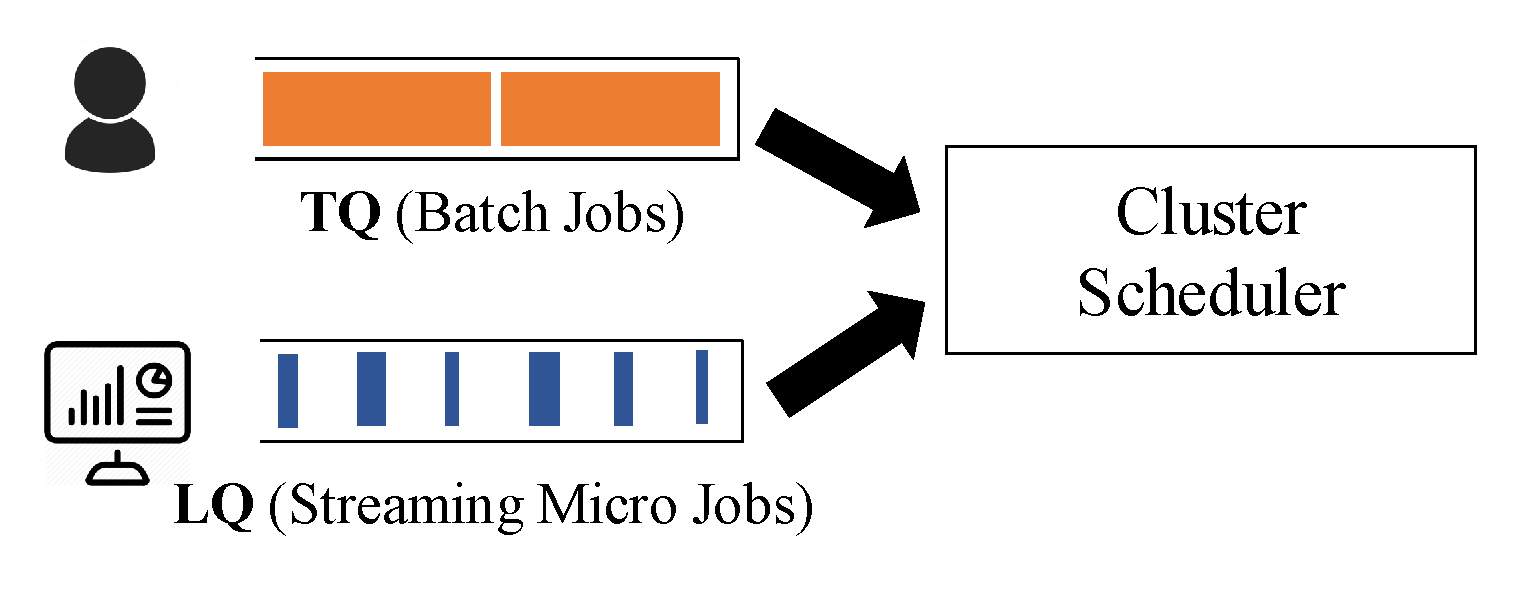
\includegraphics[width=0.8\columnwidth]{fig/queues.pdf}%
  \caption{\new{Users and automated processes submit throughput-sensitive (TQ) and latency-sensitive (LQ) to the same cluster.}}%
  \label{fig:queues}
 	\vspace{-0.1in}
\end{figure}

To address the diverse goals, today's schedulers are becoming more and more complex.
They are multi-resource \cite{drf, tetris, multiresource-mungchiang, orchestra, pacman}, DAG-aware \cite{aalo, tetris, spark}, and allow a variety of constraints \cite{late, quincy, mantri, choosy, delay-scheduling}. 
Given all these inputs, they optimize for objectives such as fairness \cite{drf, jaffe-maxmin, drfq, hdrf}, performance \cite{sjf}, efficiency \cite{tetris}, or different combinations of the three \cite{carbyne, graphene}.
However, all existing schedulers have one shortcoming in common: \emph{they force the same performance goal on all jobs while jobs may have distinct goals}, and therefore fail to provide performance guarantee in the presence of multiple types of workloads with different performance metrics. 
In fact, the performance of existing schedulers can be \emph{arbitrarily bad} for some workloads.

\begin{figure}[!t]
	\centering
	
\includegraphics[width=0.3\linewidth]{fig/b1_mov_legend} 
	\\
	\subfloat[DRF ensures instantaneous fairness, but increases the completion times of latency-sensitive jobs.]
  {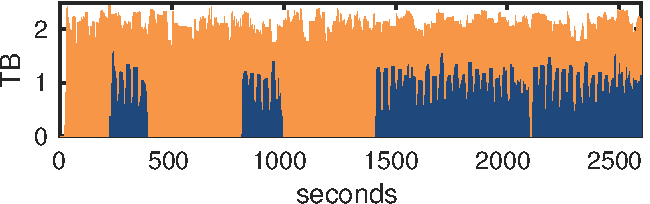
\includegraphics[width=0.85\linewidth]{fig/b1_mov_DRF_BB}\label{fig:motiv-DRF}}
	%\subfloat[DRF -- The completion time of 4 \burstq jobs are  202, 178, 715, and 719 seconds, respectively.]{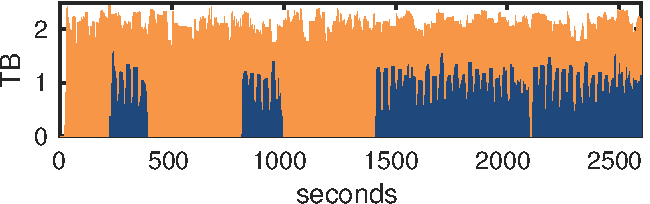
\includegraphics[width=1.0\linewidth]{fig/b1_mov_DRF_BB}\label{fig:motiv-DRF}}
	\\
	\subfloat[SP decreases completion times of latency-sensitive jobs, but throughput-sensitive batch jobs do not receive their fair shares.]
  {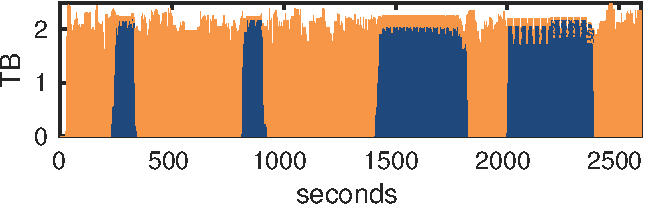
\includegraphics[width=0.85\linewidth]{fig/b1_mov_Strict_BB}\label{fig:motiv-Strict}}
	%\subfloat[Strict Prority (SP)-- The completion time of 4 \burstq jobs are  124, 121, 430, and 405 seconds, respectively.]{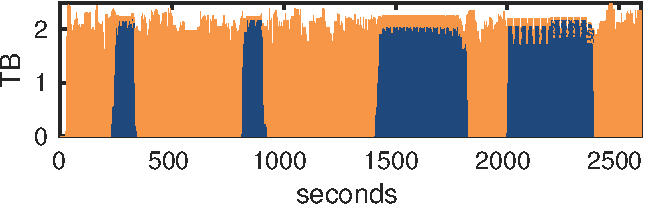
\includegraphics[width=1.0\linewidth]{fig/b1_mov_Strict_BB}\label{fig:motiv-Strict}	}
	\\
	\subfloat[The ideal solution allows first two latency-sensitive jobs to finish as quickly as possible, but protects batch jobs from latter \burstq jobs by ensuring long-term fairness.]
  {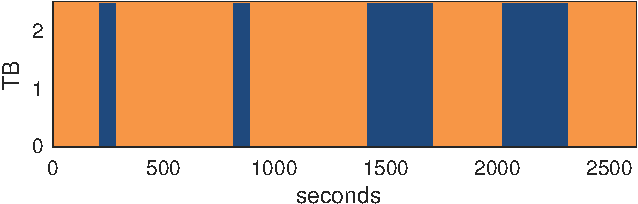
\includegraphics[width=0.85\linewidth]{fig/b1_mov_Optimum_BB}\label{fig:motiv-optimal}}	
	\caption{Need for bounded priority and long-term fairness in a shared multi-resource cluster with latency-sensitive (\burstq: blue/dark) and throughput-sensitive (\batchq: orange/light) jobs. \new{The blank part on the top is due to resource fragmentation and overheads in Apache YARN.}
    Although we focus only on memory allocations here, similar observations hold in multi-resource scenarios. \todo{put the memory (TB) instead of (TB) on the figures.}}
%    \todo{We should also have a figure showing the arrivals of LQ A.}
%    \mosharaf{Something is wrong with the third figure. Total area of blue should be the same regardless of algorithm.} 
%    \zhenhua{I didn't see the problem. The area for each arrival seems the same.}}
    %In DRF, it is unfair for the first two jobs to slow down their progress although they require very small resources. From 0 to 1400 seconds, Strict speeds up the delay-sensitive jobs from \burstq  but it later makes \batchq starving of resources because of the large jobs. \todo{change \burstq  and \batchq to \burstq  and \batchq}}
	\label{fig:motiv_ex}
		\vspace{-0.1in}
\end{figure}

Consider the simple example in Figure~\ref{fig:motiv_ex} that illustrates the inefficiencies of existing resource allocation policies, in particular, DRF~\cite{drf} and Strict Priority (SP) \cite{strict_priority} for coexisting workloads with different requirements. 
In this example, we run memory-bound jobs in 
\delete{Tez atop Apache YARN}
within a cluster of 40 nodes, where each node has 32 CPU cores and 64 GB RAM.
% 
There are two queues in the system, where each queue contains a number of jobs with the same performance goals.  
\new{Apache Hadoop YARN \cite{hadoop-fair-scheduler} is set up to manage the resource allocation among the queues.}
The first queue is for Spark streaming, which submits \delete{a number of MapReduce jobs }\new{a MapReduce job} every 10 minutes. 
We call it latency-sensitive queue (\burstq) because it aims to finish the jobs as quickly as possible.
The second queue is a throughout-sensitive batch-job queue (\batchq) formed by jobs generated from the BigBench workload~\cite{bbench} and queued up at the beginning. \batchq cares more about its long-term averaged resources received, e.g., every 10 minutes.
\todo{remove the TQ and LQ definition as they are defined in the Figure 1.}
For simplicity of exposition, all jobs are memory-bound. 
%While \burstq  tries to complete \emph{each job} as quickly as it arrives, \batchq cares more about its long-term averaged resources received, e.g., every 10 minutes.
% 
We consider two extreme classes of policies -- priority-based and fairness-based allocation -- in this example, where the former is optimized for latency and the latter for fairness.
% There are many other policies in between such as service curve and network calculus in general.
% Service curve and network calculus are often too conservative; \ie, they only admit a very small number of queues \cite{}.
Specifically, we focus on the inefficiency of DRF and SP. 
The memory resource consumption
%\footnote{The blank part on the top is due to resource fragmentation and overheads in Apache YARN.}
under these two policies is depicted in Figures~\ref{fig:motiv-DRF} and~\ref{fig:motiv-Strict}, respectively. 
We defer the discussion of other policies to Section~\ref{sec:property-analysis}. 
%\todo{We should add numbers about the completion time under two }
%\mosharaf{We should probably remove TQ and LQ names and just say latency- and throughput-sensitive jobs.}
%\zhenhua{Agreed. }

SP gives \burstq the whole cluster's resources (high priority) whenever it has jobs to run; hence, it provides the lowest possible response time. 
For the first two arrivals, the average response time is 130 seconds. 
A detrimental side effect of SP, however, is that there is no resource isolation -- \batchq jobs may not receive any resources at all! 
In particular, \burstq has incentives to increase its arrivals -- e.g., for more accurate sampling and more iterations in training neural networks -- without any punishment. 
As it does so from the third job arrival, \batchq no longer receives its fair share. 
In the worst case, \burstq can take all the system resources and \emph{starve} \batchq. 
In summary, SP provides the best response time for \burstq , but no isolation protection for \batchq at all.
In addition, SP is incapable of handling multiple {\burstq}s. 
% \zhenhua{Actually, when \burstq  increases its burst size, its response time goes worse!}

In contrast, DRF enforces \emph{instantaneous} fair allocation of resources at all times. 
During the burst of \burstq , \burstq  and \batchq share the bottleneck resource (memory) evenly until the jobs from \burstq  complete; then \batchq gets all resources before the next burst of \burstq . 
Clearly, \batchq is happy at the cost of longer completion times of \burstq 's jobs, whose response time increases by 1.6 times. 
In short, DRF provides the best isolation protection for \batchq, but no performance consideration for \burstq . 
When there are many {\batchq}s, the response time of \burstq  can be very large. 

%Therefore, it is natural to ask if we can achieve the best response time of {\burstq}s and fairness for {\batchq}s simultaneously. 
Clearly, it is impossible to achieve the best response time under \emph{instantaneous} fairness, which fully decides the allocation. 
In other words, there is a hard tradeoff between providing instantaneous fairness for {\batchq}s and minimizing the response time of {\burstq}s.
Consequently, we aim to answer the following fundamental question in this paper: \emph{how well can we simultaneously accommodate multiple classes of workloads with performance guarantees, in particular, isolation protection for {\batchq}s and low response times for {\burstq}s}? 

\begin{figure}[!t]
  \centering
  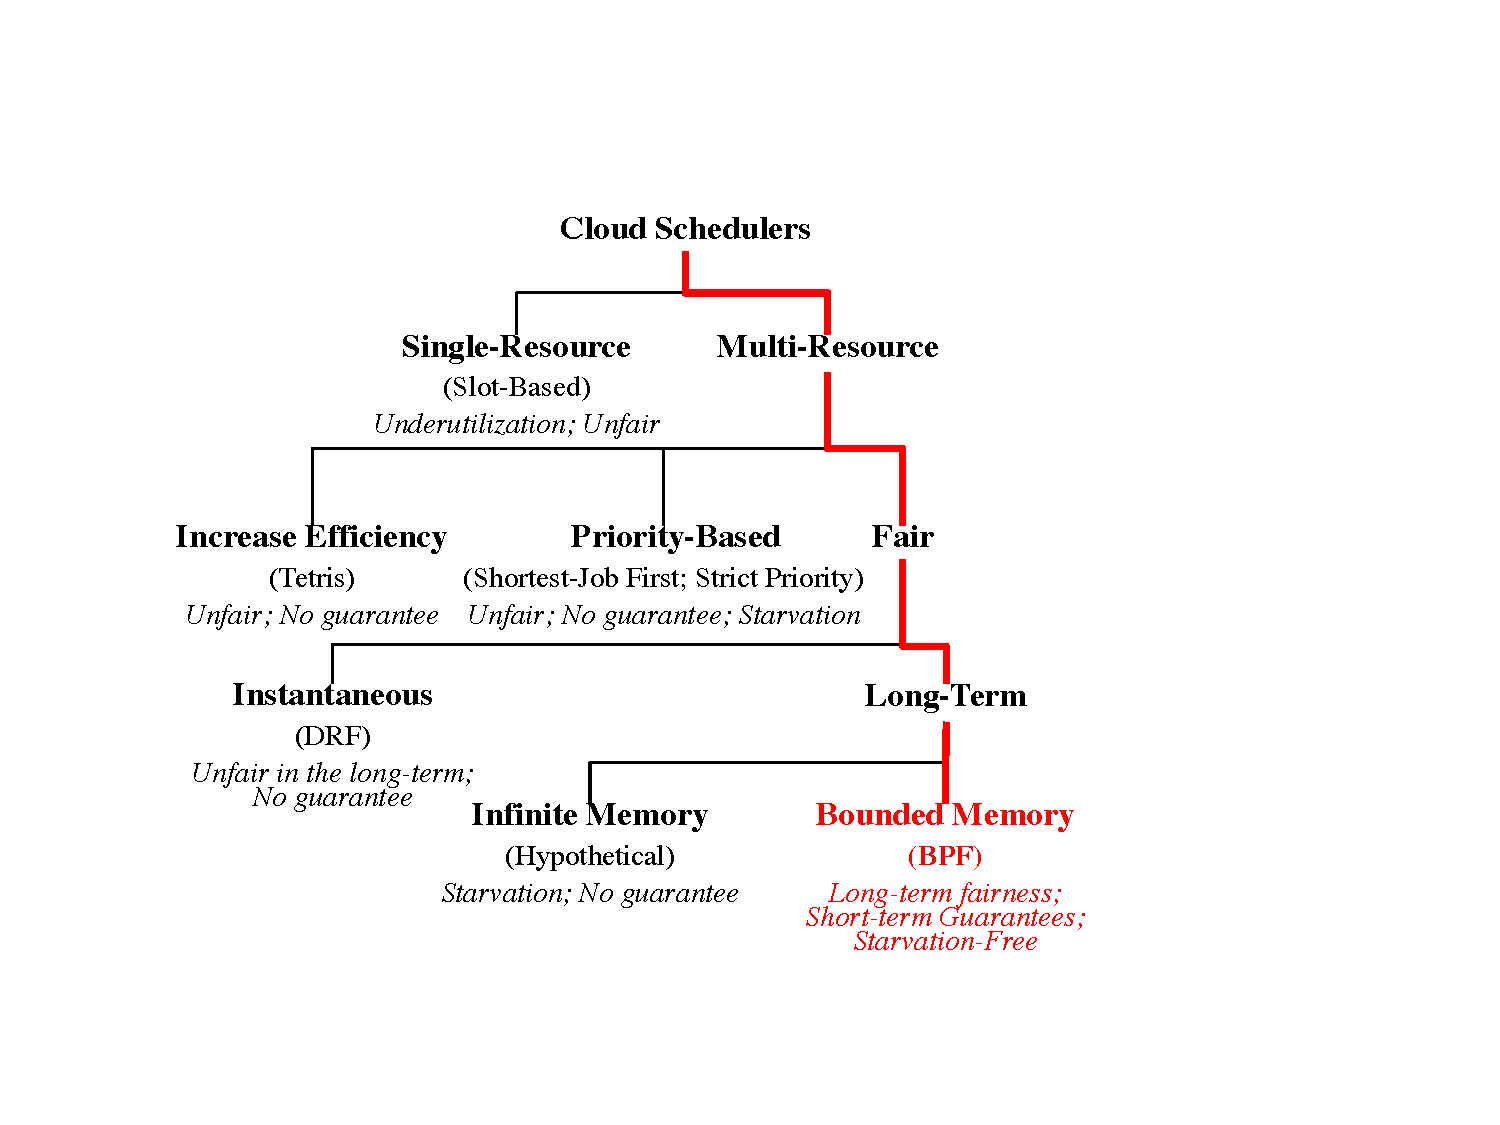
\includegraphics[width=0.85\linewidth]{fig/Design-Space.pdf}%
  \caption{{\name} in the cluster scheduling design space.}%
  \label{fig:design-space}
  	\vspace{-0.2in}
\end{figure}

We answer this question by designing \name: the first multi-resource scheduler that achieves both isolation protection for {\batchq}s in terms of \emph{long-term} fairness and response time guarantees for {\burstq}s, and is strategyproof. 
It is simple to implement and provides significant performance improvements even in the presence of uncertainties. 
The key idea is ``bounded'' priority for {\burstq}s: as long as the burst is not too large to hurt the long-term fair share of {\batchq}s, they are given higher priority so jobs can be completed as quickly as possible. 
Figure~\ref{fig:design-space} shows \name in the context of cluster scheduling landscape. 
%There are several challenges, and by solving them 
We make the following contributions.

\paragraph{Algorithm design.} We develop \name with the rigorously proven properties of strategyproofness, short-term bursts, long-term fairness, and high system utilization (\S\ref{sec:approach}). When {\burstq}s have different demands for each arrival, we further design mechanism to handle the uncertainties.

%\paragraph{Handling uncertainties.} We develop a simple yet efficient method to allow customers with significant estimation errors of their burst sizes to request the right amount of resources to satisfy their performance goals. We also highlight the difference between single-resource allocation and multi-resource allocation in the presence of estimation errors. In particular, we prove that the resource demands in the multi-resource scenario is always higher than those if resources are allocated individually unless there is no estimation error. This is true even when errors on different resources are independent. In addition, larger estimation errors lead to higher resource demands.
%\mosharaf{Didn't understand the last couple sentences, especially the phrase ``risk premium''.}
%\zhenhua{I adjusted. Let me know if it works.}

\paragraph{Design and implementation.} 
We have implemented \name on Apache YARN \cite{yarn} (\S\ref{sec:impl}).
Any framework that runs on YARN can take advantage of \name.
The \name scheduler is implemented as a new scheduler in Resource Manager that runs on the master node.
The scheduling overheads for admitting queues or allocating resources are negligibly less than 1 ms for 20,000 queues.


%
%We implement the system. One challenge is the delay in serving the bursts of {\burstq}s. \todo{Feel free to add more.}
%\mosharaf{This is probably not big enough to highlight here. Should be merged with the eval.}
%\zhenhua{That's fine. Just want to make sure it's mentioned.}

\paragraph{Evaluation based on both testbed experiments and large-scale simulations.}
In deployments, \name significantly provides up to $5.38\times$ lower completion times for \burstq jobs than DRF, while maintaining the same long-term fairness (\S\ref{sec:testbed}). 
At the same time, \name provides up to $3.05\times$ more fair allocation to {\batchq} jobs compared to SP.
%Furthermore, \name performs well even in the presence of demand variations and moderate misestimations (\S\ref{sec:sensitivity_analysis}).%\todo{sensitivity analysis regarding arrival time?}.
%\mosharaf{Not sure about talking about the preemption business here.}
%\zhenhua{Those are old texts. Feel free to edit.}

%
%\zhenhua{I'm not sure when to put the ideal allocation}
%\mosharaf{Following can be dropped.}
%The ideal allocation we target at is depicted in Figure~(\ref{fig:motiv-optimal}).
%Despite the negative result, the good news is that if we relax the instantaneous fairness to long-term fairness, both properties can be achieved at the same time. In fact, long-term fairness is good enough to provide the isolation protection to {\batchq}s. This is depicted in Figure~\ref{fig:motiv-optimal} as the ideal allocation. 
%The key idea is ``bounded'' priority for {\burstq}s: as long as the burst is not too large to hurt the fair share of {\batchq}s, they are given higher priority so jobs can be completed as quickly as possible. 
%In particular, before 1,400 seconds, \burstq 's bursts are small, so it gets higher priority, which is similar to SP. 
%After \burstq  increases its demand, only a fraction of its demand can be satisfied with the entire system's resources. Then it has to give resources back to \batchq to ensure the long-term fairness.
%
%
%=======old text=======
%
%
%Nowadays, there are multiple types of workloads with heterogeneous objectives. 
%(1) (Periodic) bursty workloads such as Spark streaming, scheduled tasks and routines. Their main goal is to minimize response time in seconds or even milliseconds.
%(2) Batch jobs. Long-term throughput measured in minutes or hours.
%(3) Interactive workloads. Non-periodic but can depend on response time, to minimize response time. Service curve is more suitable. 
%
%\thoughts{Is there a way to unify different objectives? Initial thoughts: demand can be represented by $d(t)$, where $t$ is discrete for presentation simplicity but can be easily extended to continuous case. Then $d(t)$ is nonzero at  periodic timeslots for (1), at one timeslot for (2), and at random timeslots for (3). Performance can be measured at each period for (1), after a sufficiently long interval for (2) as progress, and between consecutive arrivals for (3). Even though these workloads look different, there seems to be a way to unify them.}
%
%Under the cloud computing regime, either private or public, these workloads may share the same underlying physical infrastructure. 
%The resource contention among workloads leads to scheduling and resource allocation.
%In nowadays settings, there are multiple queues, each of which consists of a number of jobs. Each job can have multiple tasks potentially with interdependency.
%Jobs of the same queue belong to the same workload, and therefore have the same objective\footnote{A related concept is user. A user may have multiple queues, e.g., for different applications.}.
%Each queue has a weight and needs isolation guarantee. 
%Jobs may be large, e.g., for throughput-sensitive workloads. In this case, their progress can be measured by the number of tasks served within a time interval. \zhenhua{We need to clarify this to be consistent with the numerics.}
%\mosharaf{Is it possible to talk about things without introducing queues first? Then introducing queues. Btw, we should look up the Jockey paper from EuroSys 2012 carefully.}
%
%Despite the heterogeneity, start-of-the-art schedulers force the same performance goal on all workloads, which incurs inefficiency.
%
%Consider the example of a system serving both throughput-sensitive and latency-sensitive workloads. In this example, the number of tasks completed within a time interval is used to capture the progress of a throughout-sensitive batch-job queue (\batchq) \cite{tetris, carbyne, mantri, late}.
%Interactive sessions and streaming applications form latency-sensitive queues (\burstq): each \burstq is a sequence of small jobs following an ON-OFF pattern. \zhenhua{It's not really a ON-OFF pattern. It's more like a periodic arrival with deadlines...}
%For these jobs \cite{spark-streaming, spark, splunk-analysis, presto}, individual completion times or latencies are far more important than the throughput of the \burstq. 
%\mosharaf{I agree. We should get rid of this ON-OFF part. Another thing to do would be getting rid of asking for period lengths from users.}
%
%\todo{add an example to show the problem.}
%
%There are two classes of schedulers in literature, but neither of them solved the problem completely.
%\mosharaf{There is a third category that focuses on increasing utilization.}
%
%Priority-based: good for \burstq, while \batchq can be starved
%
%Fairness-based such as DRF: good for \batchq, while response time of \burstq can be arbitrarily worse compared to the optimal solution (one \burstq, $n$ {\batchq}s, $n$ goes to infinity)
%
%Other solutions: BVT, Carbyne \zhenhua{Any others? We need to discuss all of them, perhaps in the motivation section}
%\mosharaf{We may need to update the taxonomy as well.}
%
%Therefore, we ponder a fundamental question: \emph{can we enable latency-sensitive {\burstq}s and throughput-sensitive {\batchq}s to coexist, where {\burstq}s are permitted short-term resource bursts while ensuring long-term fairness between the two, as well as maximizing {\burstq}s served with resource guarantees?}
%
%In this paper, we first show that there is a hard tradeoff between instantaneous fairness and short-term resource bursts. 
%
%Then we relax the fairness notion from instantaneous one to long-term one and the key opportunity emerges: {\batchq}s do not care about allocated resources in the short term, as long as the long-term averaged resource share remains the same. This temporal flexibility allows us to accommodate bursts of {\burstq}s without hurting {\batchq}s. 
%
%However, naive admission control may result in very few {\burstq}s admitted with resource guarantees, leading to suboptimal performance for {\burstq}s even with a high system utilization.
%
%In addition, there are challenges for multi-resource allocation \zhenhua{is this trivial?} and handling the uncertainties.
%
%%\textcolor{blue}{
%%Additionally, how one reasons about system utilization becomes more complicated in the presence of both {\burstq}s and {\batchq}s. 
%%While it is relatively easy to fill the cluster with many batch jobs to achieve high utilization, {\burstq}s often have higher value and are harder to accommodate with resource guarantees. 
%%Compared to a simple solution that rejects most of {\burstq}s and/or serves them with best efforts, system operators are likely to prefer to maximize the {\burstq}s served with resource guarantees, which leads to more predictable performance. %We call the resources allocated to {\burstq}s with resource guarantees {\burstq} utilization.
%%%}
%%}
%%
%%
%%The challenges are \zhenhua{we should add some key messages from theoretical results. My current thoughts are: BG and LF seem not very challenging given the opportunity we discussed in the last paragraph, so we should focus on strategyproofness and (LQ) utilization. Xiao, as you have some concerns regarding the strategyproofness, can you write down your thoughts here? If BPF in the current form is strategyproof, then we should highlight some other alternatives are not, similar to our HUG paper. Otherwise, we should improve BPF and use the current version as the example. I can write something along our NSF proposal regarding the tradeoff between progress and utilization. I looked into our HUG paper, and it seems the intro has quite a few strong points, such as DRF's utilization can be arbitrarily low, naive work conservation can lead to worse utilization, etc. Meanwhile, the elastic demand is very clear. We should try to do something similar. }
%%
%%
%%
%%\textcolor{blue}{
%%The need to separate throughput- and latency-sensitive job queues in big data clusters is akin to the classic networking problem of supporting throughput-sensitive flows and latency-sensitive realtime communication on network access links \cite{cbq, intserv-hierarchy, hfsc, cruz-sc}.
%%The key difference between the two is the multi-resource nature of cluster scheduling and challenges arising from it. 
%%We aim for a solution that can be applied to multi-resource clusters.
%%}
%
%\textcolor{blue}{
%%\todo{five properties, but some are missing below.}
%In this paper, we first explore opportunities and challenges in achieving four desired properties in this context (\S\ref{sec:motivation}): (i) allowing {\burstq}s to enjoy short-term high resource usage during their ON periods to minimize \emph{individual} job response times; (ii) maintaining the same \emph{long-term} fairness as existing multi-resource fair allocation policies by preventing arbitrarily large bursts; (iii) maximizing system utilization and {\burstq}s served with resource guarantees; %\new{(iv) It is better off sharing than using static sharing}. 
%and (iv) the policy needs to be strategyproof because otherwise {\burstq}s may lie about their demands to gain more resources. 
%}
%
%\subsection*{Contributions}
%
%\paragraph{Algorithm development.} properties with rigorous proofs: strategyproofness, short-term bursts, long-term fairness, system utilization
%
%\paragraph{Design and implementation.} any challenges here? The slow start problem that Tan is currently working on is one potential.
%
%\paragraph{Evaluation based on both testbed experiments and large-scale simulations.}
%In deployments, \name significantly provides up to $5.38\times$ (totally 9 queues in a cluster) faster performance with smaller variation for \burstq jobs than DRF, while maintaining the fairness among the queues (\S\ref{sec:testbed}). 
%\name protects the {\batchq} jobs up to $3.05\times$ compared to SP.
%Furthermore, \name performs well even in the presence of moderate misestimations of task demands and without preemption allowed (\S\ref{sec:sensitivity_analysis})\todo{sensitivity analysis regarding arrival time?}.
%
%\section{Motivation}
%
%\mosharaf{If we could talk about some numbers that'd be good. Of course, we don't have any real traces ourselves. One possible option is going through existing works and see if they mention any high-level characteristics that we can use.}
%\zhenhua{I agree. While searching for existing work, we can start from some simple examples as we did in the HUG paper, which is well received.}
%
%\subsection{Problem Formulation}
%
%\subsection{Desired Properties}
%
%\subsection{Challenges and Inefficiencies of Existing
%Allocation Policies}
%
%SP
%
%DRF
%
%BVT
%
%Carbyne
%
%others?
%
%\subsection{Hard tradeoff between instantaneous fairness and bursty accommodations}
%
%\subsection{Naive admission control results in few {\burstq}s admitted with performance guarantee}
%
%\subsection{Estimation errors matter}
%
%
%\section{\name: analytical results}
%
%The \name algorithm
%
%long-term fairness
%
%burst guarantee
%
%Pareto efficiency
%
%strategyproofness
%
%\section{Stochastic optimization to handle the uncertainties}
%\zhenhua{Xiao is working on this}
%
%Model
%
%Algorithm
%
%
%\section{System design}
%
%Reducing overheads from creating containers. \zhenhua{Tan is looking into this}
%
%\section{Evaluations}
%
%\zhenhua{Tan, can you add the current figure list here?}
%
%\todo{Everyone, please add to the figure list addition figures that may help.}
%
%
%We discuss related work in Section~\ref{sec:related}.

%\mosharaf{A list of three contributions? Problem formulation, Algorithm and its properties, and full system evaluation and thorough eval.}


\section{Background \& Motivation}
\label{sec:background}

\subsection{Interchangeable resources}
\label{sec:speedup}

\desc{GPUs are designed for heavy computing applications}

% GPUs become more important than ever because of the rapid increase in compute-intensive applications.
Modern GPUs are not only graphics processors but can also process massive data in parallel using hundreds or thousands of reduced-instruction-set cores.
Consequently, GPUs have been in wide use for deep-learning applications like image classification, video analytics, speech recognition, and natural language processing \cite{image_classfication_deep,image_classification_cnn,cuda_video_coding, nn_nlp, deep_cnn_nlp}.

% \begin{figure}[h]
% 	\centering
% 	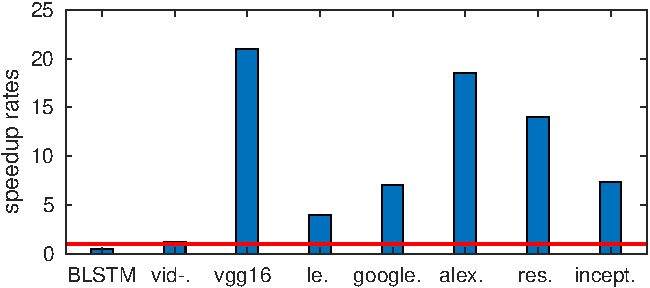
\includegraphics[width=1.0\linewidth]{figs/speedup_rates} \vspace{-0.2in}\caption{Jobs have different speedups from Nvidia K80 GPU versus Intel Xeon E5 2.4 GHz 20-core CPU.}\vspace{-0.1in}
% 	\label{fig:speedup_rates}
% \end{figure}

\desc{GPUs are not always cost effective.}

Different jobs obtain distinct speedups by using GPUs versus CPUs, as shown in Figure~\eqref{fig:speedup_rates}. The speedup rate is how much GPU can reduce the job processing time, i.e., job processing time on a particular CPU divided by that on one GPU. 

While GPUs are generally more efficient for machine learning jobs (with a speedup rate larger than 1), they are more expensive. Figure~\eqref{fig:cost_perf} shows that the normalized costs (the cost ratio between GPUs and CPUs divided by the speedup) vary a lot. When the normalized cost is greater than 1, using GPU is not cost-effective. 

\begin{figure}[h]
	\centering
	%    
\includegraphics[width=0.6\linewidth]{fig/b1i3_res_usage_legend} 
	\subfloat[Speedups from Nvidia K80 GPU versus Intel Xeon E5 2.4 GHz 20-core CPU.] {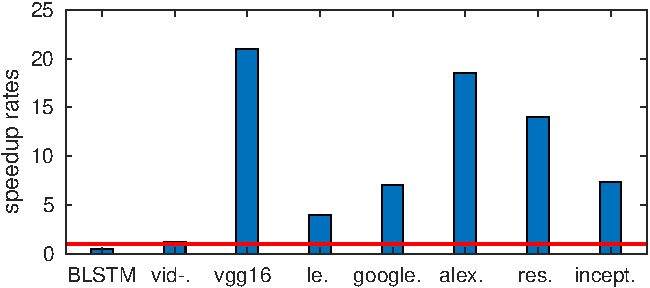
\includegraphics[width=1.0\linewidth]{figs/speedup_rates} \label{fig:speedup_rates}}    \hspace{0.0in}
	\subfloat[Normalized costs using CPUs (c5.large) versus GPU node (p2.xlarge) on EC2] {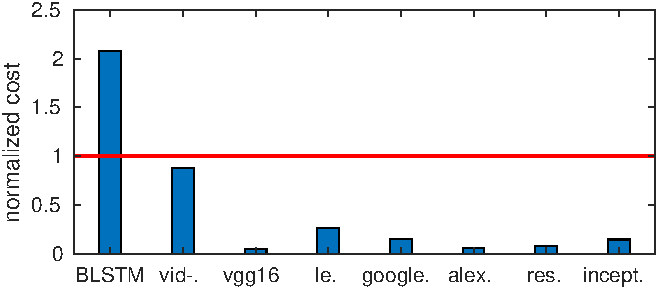
\includegraphics[width=1.0\linewidth]{figs/cost_perf_cloud} \label{fig:cost_perf_cloud}} 
	\caption{GPUs provide distinct speedup and cost-effectiveness.}
	\label{fig:cost_perf}
\end{figure}



%Despite their increasing popularity, GPUs are not always cost effective.
%Figure~\ref{fig:cost_perf} shows normalized costs of CPU and GPU on different benchmarks running on TensorFlow.
% We consider both their off-the-shelf prices and prices on Amazon EC2.
% The normalized cost is the ratio of the GPU price and CPU price, further divided by the speedup rate. The speedup rate is how much GPU can reduce the job processing time, i.e., job processing time on a particular CPU divided by that on one GPU. 
% While GPUs are generally more efficient for machine learning jobs (with a speedup rate larger than 1), they are more expensive. 
% If the normalized cost is more than 1, using GPU is not cost-effective. 

The ineffectiveness of using GPUs in some jobs is due to several reasons.
Although TensorFlow can speedup the performance of CNN models like VGG16, ResNet50, AlexNet, and Inception3 using GPUs \cite{tensorflow-benchmark}, it does not work well with memory networks like Bidirectional LSTM (Bi-LSTM) \cite{deep-learning-cpu-gpu-benchmark}.
RNN models are often updated for each training example for the dependency between two time frames which creates difficulty for parallel computing \cite{huang2013accelerating}.
For the large data input like video-analytics (vid.) \cite{keras-video-classifier}, GPUs are not effective due to the bottleneck in memory and I/O. Therefore, CPUs are preferred for the pre-processing of the video data for the deep learning models.

%\begin{figure}
%	\centering
%	\includegraphics[width=0.7\linewidth]{figs/beta_mov}
%	\caption{Tensorflow jobs have different speedup rates on GPUs (Nvidia K80) vs CPU Xeon E5 2.3Gz 20 cores.}
%	\label{fig:beta_mov}
%\end{figure}




% \desc{CPU applications are still dominant in CPU/GPU clusters}
% We also observe that CPU-only applications are still dominant in most clusters.
% Traditional for-CPU applications have been developed over many years, and it is impractical to convert all these applications for GPUs.
% Furthermore, if the applications are I/O bound, GPUs are not useful.
% For example, database queries are often bound by disk, memory, or network I/O \cite{li2016hippogriffdb}.
% Finally, GPU memory is relatively small; thus it can be a bottleneck for memory-bound applications.
% If the applications do not require much computation, developers will not convert them into GPU applications.
% Although GPU demand is increasing, the load from GPU applications are still small compared to the CPU applications.
%\todo{find the ratio of CPU load vs. GPU load.}

%%% We cannot argue GPUs are not cost effective because speed-up to costs rates are still high as CPU with more CPU cores are also very expensive.
%GPUs may not be cost effective.
%We define the performance-cost ratio as $\frac{\text{speed-up rate}}{(\text{price of GPU}/\text{price of CPU})}$.
%Nvidia shows that Nvidia Tesla K80 can speed-up up to 10x against Intel Xeon E5v3 3.6 Ghz \cite{gpu-k80-speedup}.
%The price of GPU Nvidia Tesla K80 is \$3990 \cite{} while the price of Intel Xeon E5v3 3.6 Ghz is \$363.5 \cite{}.
%
%\begin{figure*}[h]
%    \centering
%    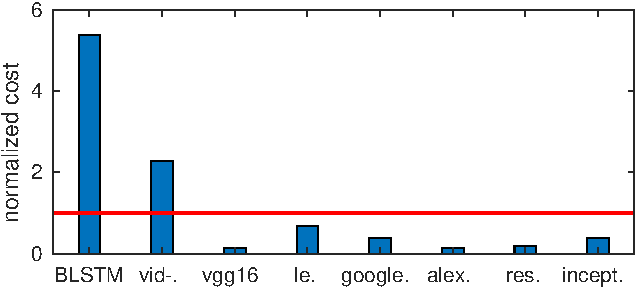
\includegraphics[width=1.0\linewidth]{figs/cost_perf_physical}
%    \caption{Performance-cost ratios show GPUs are not cost-effective because most of ratios are less than 1. Nvidia claims that the speed-up rates of using Nvidia Tesla K80 speeds up 1-10x \cite{gpu-k80-speedup} against Intel Xeon E5v3 3.6 GHz. The price of GPU is \$3990, while the price of CPU is \$363.5.}
%    \label{fig:cost_perf_physical}
%\end{figure*}

\desc{Traditional CPU clusters are low in utilization that gives space for running GPU workloads on CPU.}

In addition to being cost-effective for some jobs, CPUs are often under-utilized.
To this end, we analyzed the Azure Public Dataset \cite{AzurePublicDataset}, which recorded CPU utilization of 5,958 users over 30 days.
We found that more than 90\% users use less than 20\% of their allocated CPU (Figure~\ref{fig:avg_util}).
Because jobs can be executed on CPUs when GPUs are busy, we could utilize the available CPUs before spending a lot in adding more, expensive GPUs.

\begin{figure}[h]
	\centering
	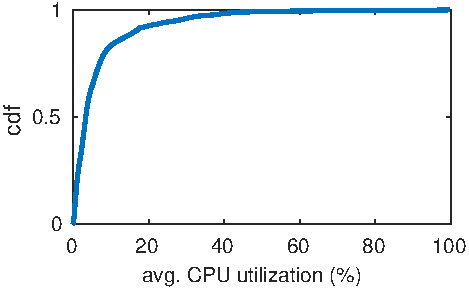
\includegraphics[width=0.8\linewidth]{figs/avg_util}
	\caption{Most of Microsoft Azure users (92.6\% of 5,958 users) have average CPU utilization under 20\%.}
	\label{fig:avg_util}
\end{figure}


\desc{There are interchangeable resources.}

% Thanks to frameworks like TensorFlow \cite{tensorflow}, machine learning applications can run on both CPUs and GPUs.
% Meaning, GPUs can be interchanged with CPUs and vice versa.
% Interchangeable resources like CPUs and GPUs are not rare in large heterogeneous clusters: 
% Heterogeneous CPUs can be interchanged because a more powerful CPU can give better performance than the weaker ones.
% Similarly, one can interchange different network interfaces with different bandwidths, and SSDs with HDDs.

%\subsection{Limitations of current schedulers for CPU/GPU clusters}

\desc{Cannot handle interchangeable resources.}

Unfortunately, existing cluster schedulers do not support interchangeable resources (Table~\ref{tbl:schedulers}) and it is not easy to extend existing schedulers to handle both performance and fairness in the presence of multiple configurations.
Usually, jobs are pre-configured to run on either CPUs or GPUs, therefore systems do not have the flexibility to determine whether to place a job on CPU or GPU. For example, jobs preferring to use GPUs may wait in the GPU queue for a long time, even if CPUs are available and could be a better option in some cases.
Moreover, the configurations are pre-configured by users, who may not know the system-level information to choose the right configurations.


\begin{table}[h]	
	\caption{Resource allocation systems that support GPUs.}
	\label{tbl:schedulers}
	\begin{tabular}{|p{3.5cm}|c|c|}
		\hline
		Systems &  Schedulers & Interchangeability \\ \hline \hline		
		Apache YARN \cite{yarn}    & Fair, DRF & No    \\ \hline
		Kubernetes \cite{kubernetes} & Best effort & No \\ \hline
		Apache Mesos \cite{mesos}   &  DRF          & No  \\ \hline
		Apache Spark \newline (Standalone Mode) \cite{spark}   &  Fair         & No  \\ \hline
	\end{tabular}\vspace{-0.2in}
\end{table}

\desc{Fixed Resource placement is not efficient}

%Since the resource configuration of a job is fixed before its submission, resource interchangeability becomes impossible.


\subsection{Inefficiencies of strawman solutions}
\label{sec:perf-strawman}
%\xiao{new idea: consider the load. When the load is low, actually both MEC and JSQ+ are optimal. But when the load increases, there is a problem. Our approach shirinks to JSQ+ or MEC when the load is low, but when load increases, we have better performance}


\desc{Problem Definition}
To better understand the shortcomings of simplistic heuristics, let us consider a simple setup. 
Assume there are $n$ users sharing a system consisted of interchangeable resources, where each user submits their jobs over time. 
Each job has up to $k$ configurations to run. 
For simplicity of presentation, we restrict our attention to two configurations, i.e., the GPU and the CPU configurations; however, our algorithm and analysis can be readily extended to more configurations, and  different scenarios such as networking interfaces or storage devices. 
A job scheduler for interchangeable resources needs to decide 
(i) the configuration to use for each job and 
(ii) the order of jobs to optimize performance and fairness objectives. 

By default, we do not allow preemption because it is not well supported in many systems such as Kubernetes. 
Even if it is supported, the overhead of migration is often very high. 


%% tan: deletes this example because it does not help.
\del{
Consider a simple example where there are 1 CPU consisted of 32 cores and 1 GPU in the system. 
Each job has two configurations: either the whole CPU or the whole GPU (with a small amount of CPU, e.g., less than a core, to ensure normal execution). 
There are two users. 
User 1 has 5 jobs, each takes 10 minutes to finish on CPU, and 5 minutes on GPU. User 2 has 5 jobs requires 40 and 10 minutes on CPU and GPU, respectively. 
If we want to minimize the average job completion time (JCT), the optimal solution is to put all jobs of user 1 on CPU and all jobs of user 2 on GPU, resulting in an average JCT of 30 minutes. 
}


%processing time on CPU, or 5 mins on GPU, while Job 2 requires either 40 mins processing time on CPU or 10 mins on GPU. If we try to minimize the average completion time, then clearly we should use GPU for job 2 and CPU for job 1.





%Each version will use corresponding GPU or CPU as the computational resource, and each job can only pick one configuration. Assume every job has the same configuration settings, but the processing time on different resources are different, and we assume the processing time is known. The goal is to decide the configuration for each job and then schedule the jobs to reach a better performance and fairness output.

While (ii) has been studied extensively in existing work~\cite{drf,drfq,carbyne,tetris,hug}, (i) is the new challenge. 
In this section, we revisit existing algorithms for this new problem to illustrate their inefficiencies and demonstrate why we need new algorithms. 
In addition, we show that strawman solutions may lead to poor performance, highlighting that designing a new algorithm is challenging.






%In the following subsection, we will consider performance (in terms of job completion time) and fairness seperately. We will see that a strawman solution fails to solve this problem -  and in most of the time, far from optimal solution.

%\subsubsection{Performance}

We focus on performance in this section, in particular, minimizing the average job completion time (JCT). Fairness is discussed in Section~\ref{sec:fairness}.  

\desc{Each job use its most effective resource}

%For the problem described above, if our goal is to minimize average completion time, the problem is in P if we assume all jobs arrives at time 0. if they arrive over time, then the problem becomes strongly NP-Hard, even if we allow preemption. Before we discuss our polynomial algorithm in section xxx, we start with heuristics and show why they did not work.


The first approach we consider is Most Effective Configurations (MEC): the scheduler asks users to pick one configuration for each job and the scheduler is only responsible for the job ordering and placement. 
Under this approach, the load on CPU and GPU can be largely unbalanced. For instance, if all jobs favor GPUs, no users would pick the CPU configuration, resulting in arbitrarily low utilization of CPU, and vice versa. 
Actually, if there are $k$ interchangeable resources, this approach may result in $k-1$ of them unused. 

The under-utilization of resources has profound impacts on job completion time, especially when the system load is high. For instance, assume all the GPUs together can finish 10 jobs/minutes on average and all the CPUs can finish 10 jobs/minutes possibly with longer processing time for each job. Then if the arrival rate is 15 jobs/minutes, the waiting time when we only use GPUs would keep increasing. Under the ``heavy traffic'' situations, low utilization results in arbitrarily large job completion time. 
%\del{, and these situations are exactly when we greatly need thoughtful scheduling algorithms}.
Therefore, \emph{picking the most effective configuration for each job may result in low utilization and high waiting time}.

%This approach is not optimal, as the load of CPU and GPU can be largely unbalanced, especially for machine learning jobs. For example, if for all jobs, the processing time on GPU is always shorter than CPU, then of course people would choose using GPUs in a shared cluster. While GPU is fully utilized, CPUs are barely used. So the performance can be as bad as the computational power between total GPUs and total CPU cores. For example, if they have the same computational power, then the degeneration can be as much as 50\%.

\desc{users see the load}

The inefficiency of MEC is because the configuration selection does not take into consideration the current system load. Therefore, the second approach is a modified Join the Shortest Queue (JSQ+). 
Assume users know the current waiting time on each resource in real time. On the arrival of a job, the scheduler picks the resource that has the shortest completion time, i.e, the sum of waiting time and the processing time of the job on the corresponding resource. 
In this way, loads on different resources can be more balanced because as the load on some resources increases, their longer waiting time would encourage new jobs to be placed on other resources. 
Note that it is different than the vanilla joining the shortest queue. 
For instance, if a job has the processing times of 10 minutes and 40 minutes on GPU and CPU, respectively, and the waiting times on GPU and CPU are 40 and 20 minutes, respectively.
Although CPU has a shorter waiting time, this job pick GPU because it is much more efficient on GPU, resulting in a completion time of 50 minutes.
If the job was placed on CPU, the completion time would increase to 60 minutes.

%reports back the current node on different resource - so the user can choose whichever node that has the shortest expected finishing time if the job will be running on that node. 

\emph{The key drawback of JSQ+ is that it is short-sighted}: each job attempts to minimize its own completion time without considering the impacts on later jobs. 
Here is an example with 2 CPUs and 2 GPUs. Assume there are 4 jobs, all arrive at the beginning but in the order of Job 1, 2, 3, 4. The processing time can be show in a matrix: 
$$
P = \begin{bmatrix}
40 & 50 \\
40 & 50 \\
40 & 80\\
40 & 80\\
\end{bmatrix}
$$
In this matrix, the $i$-th row consists of job $i$'s processing times on GPUs and CPUs, respectively. For instance, the first row means Job 1 needs 40 minutes on GPU or 50 minutes on CPU.

Under JSQ+, Job 1 first picks a GPU, and then Job 2 picks the other GPU.
After that, Job 3 and Job 4 have no choices but to pick CPUs, as shown in Figure~\eqref{fig:JSQ_ex} with an AJCT of 60 minutes.
%\xiao{This may not be true, as Job 3 and 4 can choose to join the GPU queue and wait instead of using CPU directly}
Clearly, the optimal solution is to put Job 3 and 4 on GPUs and Jobs 1 and 2 on CPUs, which can reduce the AJCT from 60 minutes to 45 minutes as Figure \eqref{fig:JSQ_ex_opt}.

\begin{figure}[h]
	\centering
%	{
\includegraphics[width=0.7\linewidth]{figs/JSQ_ex_legend} \label{fig:JSQ_ex_legend}}    \hspace{0.0in}
	\subfloat[JSQ+] {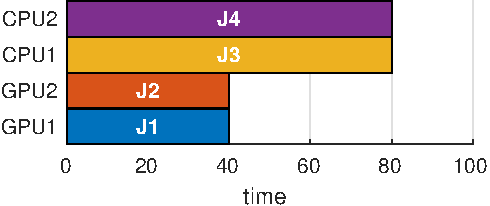
\includegraphics[width=0.7\linewidth]{figs/JSQ_ex} \label{fig:JSQ_ex}}    \hspace{0.0in}
	\subfloat[Optimal] {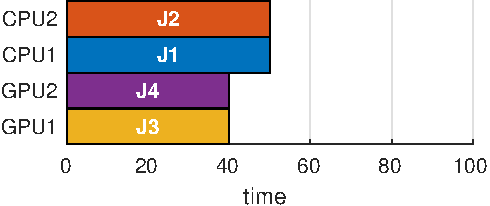
\includegraphics[width=0.7\linewidth]{figs/JSQ_ex_opt} \label{fig:JSQ_ex_opt}}    \hspace{0.0in}	
	\caption{Under JSQ+, Job 1 and 2 are scheduled on GPU, while Job 3 and 4 are scheduled on CPU. In contrast, \name runs Job 3 and Job 4 on GPUs because they have higher speedup on GPUs. } %\tanle{We don't need 4 jobs in the motivation examples. Should I make it to two jobs or vary the lengths a bit?}}
	\label{fig:JSQ}
\end{figure}

%Clearly, this is not an optimal solution, as there is more gain by scheduling Job 3 and 4 to GPUs.


\desc{System pick configuration}

The sub-optimality of these two strawman solutions implies that we cannot just let each user pick her own job configurations, even if users are equipped with the current system load information. 
Therefore, the scheduler needs to coordinate the decisions, where Shortest Job First (SJF) is widely used.
%So now we consider a centralized approach by comparing all configurations between jobs. 

When there are multiple configurations for each job, we can extend SJF to SJF+ to handle jobs with multiple configurations: for each type of resource, maintain a queue of all available jobs. The jobs are sorted based on the processing time on this resource, e.g., GPU, in an increasing order. Whenever a resource becomes available, schedule the first job in the corresponding queue to this resource and remove the job from all queues. When multiple resources are available at the same time, first schedule a job to the one with shorter processing time. 

This algorithm is optimal when there is only 1 configuration~\cite{cobham1954priority}. 
%\todo{Xiao, can you add the citation?}
When there are more than 2 configurations, however, the performance can be \emph{arbitrarily bad}. Consider the following example:

$$
P = \begin{bmatrix}
10 & 20\\
10 & 20 \\
20 & 90\\
20 & 90\\
\end{bmatrix}
$$


\begin{figure}[h]
	\centering
%	
\includegraphics[width=0.7\linewidth]{figs/SJFplus_ex_legend} \hspace{0.0in}
	\subfloat[SJF+] {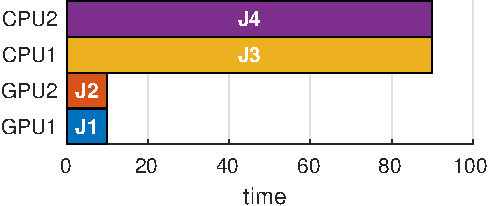
\includegraphics[width=0.7\linewidth]{figs/SJFplus_ex} \label{fig:SJFplus_ex}}    \hspace{0.0in}
	\subfloat[Optimal] {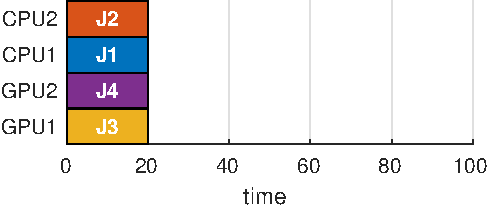
\includegraphics[width=0.7\linewidth]{figs/SJFplus_ex_opt} \label{fig:SJFplus_ex_opt}}    \hspace{0.0in}
%	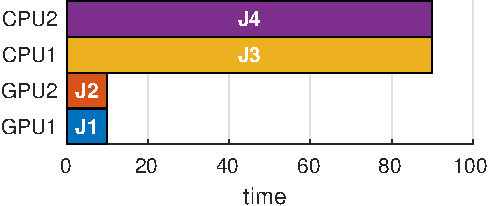
\includegraphics[width=0.8\linewidth]{figs/SJFplus_ex}
	\caption{Under SJF+, Job 1 and 2 are scheduled on GPU, while Job 3 and 4 are placed on CPU. In contrast, \name places Job 3 and Job 4 on GPUs because the time reductions on GPUs of these two jobs are larger.}
	\label{fig:SJF}
\end{figure}


Under SJF+, there are two queues for GPU and CPU, respectively. The order in both queues is Job 1, Job 2, Job 3, Job 4. Therefore, Job 1 and 2 are placed on GPUs first. Then Job 3 and 4 are scheduled on CPUs. This is shown in Figure~\ref{fig:SJF}, resulting in an AJCT of 50 minutes. 
%Job 3 and 4 are large jobs and they have more gains by putting them into GPUs, however, because of the non-idle property of SJF scheduling, Job 3 and 4 are forced to be scheduled on an inefficient resource.
In contrast, the optimal solution places Jobs 3 and 4 on GPUs and Jobs 1 and 2 on CPUs, reducing the AJCT to 20 minutes. 
The root cause is while Jobs 3 and 4 are longer (disadvantage in SJF+), the processing time reduction of using GPU is much larger (overlooked by SJF+).


To summarize, when jobs have multiple configurations, even if jobs arrive at the same time, the problem is more challenging than that with single configuration because we need to consider the processing time reduction among different configurations, which may contradict with other factors, e.g., the length of the job. Therefore, algorithms that perform well for single configuration job scheduling may result in arbitrarily bad performance in the new problem.  

%with 2 configurations for each job, all existing heuristics failed to provide a good guarantee, even for the simplest case. The root is that, it seems to have more gains, we should schedule large jobs on efficient resource, but from traditional scheduling perspective, to minimize average completion time, we should start with smaller jobs. 


In \S\ref{sec:alg}, we will provide a network algorithm, and show its optimality for average job completion time.





% \subsection{Illustrations of \name}

% \desc{Strawman solutions do not work.}

% To handle interchangeability, a strawman solution would equally shares the resources among users and then places the jobs into resource in the best-effort manner.
% To illustrate the inefficiency of the strawman solution and the potential of \name, we create an simple example in Table \ref{tbl:mov_example}.
% There are 2 users, i.e., User 1 and User 2.
% Each user has 3 jobs.
% Each job can execute either on CPU or GPU with different completion times.
% The GPU/CPU speed-up rates of jobs are different.
% 6 jobs are queued up at the beginning.

% \begin{table}[H]    
% 	\caption{Motivation example.}
% 	\label{tbl:mov_example}
% 	\begin{tabular}{|c|c|c|c|}
% 		\hline
% 		User & Job ID & Compl. on GPU & Compl. on CPU \\  \hline \hline
% 		User 1 & 1 & 3 & 4 \\  \hline
% 		User 2 & 2 & 3 & 3 \\  \hline
% 		User 1 & 3 & 1.5 & 4 \\  \hline
% 		User 2 & 4 & 2 & 3 \\  \hline
% 		User 1 & 5 & 1 & 2 \\  \hline
% 		User 2 & 6 & 1.5 & 2 \\  \hline
% 	\end{tabular}
% \end{table}

% Figure \ref{fig:motivation_example} compares the strawman solution and \name.
% The strawman solution in Figure \ref{fig:motivation_example_1} equally shares CPU and GPU for two users and places the jobs in CPUs and GPUs.
% The average completion time of 6 jobs in Figure \ref{fig:motivation_example_1} is $\frac{20}{6}$.
% The strawman solution fully utilizes the resources but its performance is far from optimal.
% Figure \ref{fig:motivation_example_2} illustrates our solution that is clearly better than the strawman one.
% The average completion in Figure \ref{fig:motivation_example_2} is $\frac{13}{6}$ that achieves $35\%$ performance improvement.

% \begin{figure}[H]
% 	\centering
% 	% 3+4+3+5+2+3
% 	\subfloat[Fair share \& Best effort] {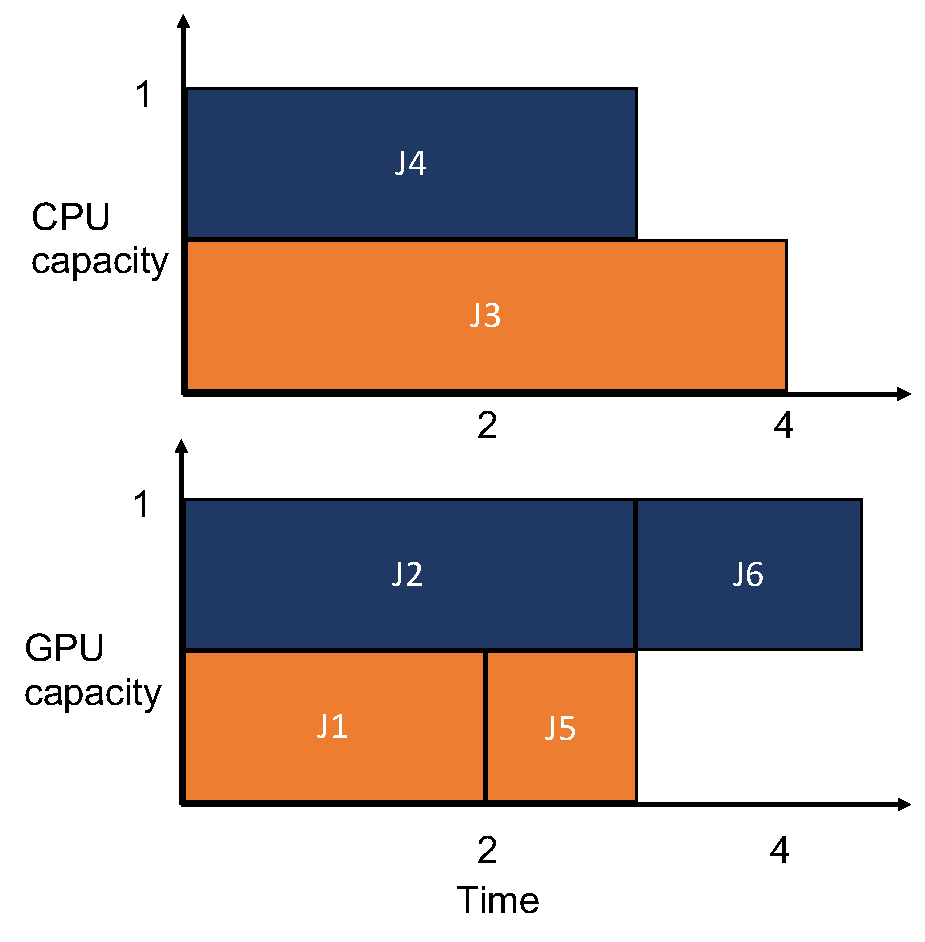
\includegraphics[width=0.45\linewidth]{figs/motivation_example_1} \label{fig:motivation_example_1}} 
% 	% 3+2+1.5+3+1+2.5
% 	\subfloat[\name allocation \& scheduling ]{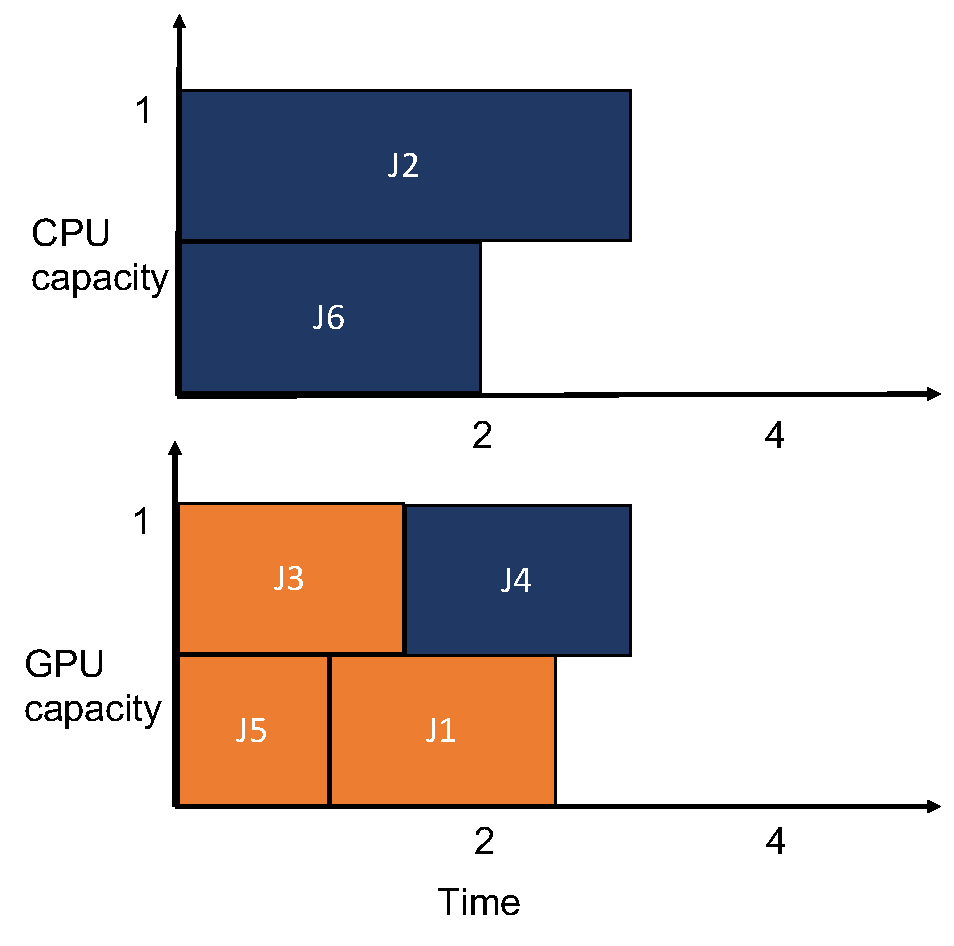
\includegraphics[width=0.45\linewidth]{figs/motivation_example_2} \label{fig:motivation_example_2}}
% 	\caption{Opportunities for job scheduling in CPU/GPU clusters.
% 	Figure \ref{fig:motivation_example_1} depicts the allocation of the strawman solution using fair-share and best-effort scheduling in the FIFO maner.
% 	Although the strawman solution fully utilizes resources, it does not give the optimal solution.
% 	Meanwhile, \name exploits the interchangeability between CPUs and GPUs to improve 35\% performance.}
% 	\label{fig:motivation_example}
% \end{figure}

% \xiao{Motivation starts here} \\
% As our goal is manifold: fairness, efficiency and performance, we show that current existing schedulers and algorithms fail to provide satisfiable result in at least 1 or more aspect.



%This approach works well in the offline case where we can perfect measure the $\beta$. If the $\beta$ is properly choose, we can prove that this algorithm is Pareto-efficient, Envy-free and sharing-incentive. 

%However, under online case, we can not get perfect $\beta$, and the estimation will be changing overtime, so the dominant share of all users are fluctuating, thus those properties can hardly hold in online case.

% \subsubsection{Efficiency}

% In traditional multi-resource allocation problem, the efficiency, or the system utilization is often optimized based on some greedy 'packing' heuristics. As long as the resource is not wasted at every time slot, we should observe a better makespan, so that the efficiency will be improved.  However, under \name, this is no longer true due to job placement onto an improper computation resource. Consider the following example:

% Assume the cluster size is (24 CPU cores, 2 GPUs and 48 GB memory) there is only 1 user in the system and the user has 2 different categories of jobs. 9 jobs are from Type A, which require 8 CPU cores and 8 GB memory, with 10 units processing time and 1 GPU and 2 GB memory with 3 units processing time. 2 jobs are from Type B, which require 16 CPU cores and 16 GB memory, with 8 units processing time on CPU and 1 GPU and 2 GB memory with 30 units processing time.

% The comparison of a packing scheduler and a non-packing scheduler is shown at figure \ref{fig:efficiency}.
% \begin{figure}
% 	\centering
% 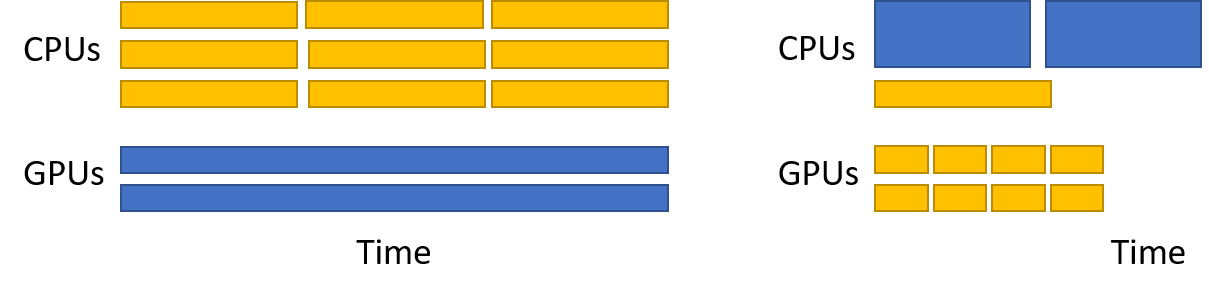
\includegraphics[width=0.8\linewidth]{figs/efficiency}
% 	\caption{Perfect packing does not leads to good utilization. The makespan for left figure is 30, and it is 16 for right figure with imperfect packing.}
% 	\label{fig:efficiency}
% \end{figure}


% \subsubsection{Performance}
% The performance evaluated for a user is based on the average completion time of all jobs from that user. Usually for this objective function,  the widely applied heuristic policy is shortest  job first - simply sort all jobs and schedule the job with shortest processing time. We show that simple vanilla greedy SPT algorithm would also face challenges under our interchangeable settings.

% Similar to previous setting, assume we have a cluster of size (24 CPU cores, 2 GPUs and 48 GB memory) and there is only 1 user in the system, so we don't have to consider fairness. There are 2 types of jobs, all of them have identical job demand but have different processing time. For type A jobs, they require 8 time units on both CPU and GPU. For type B jobs, they require 10 units on GPU and 20 units on CPU. The schedule for SPT and optimal is shown at Figure \ref{fig:performance}.

% \begin{figure}
% 	\centering
% 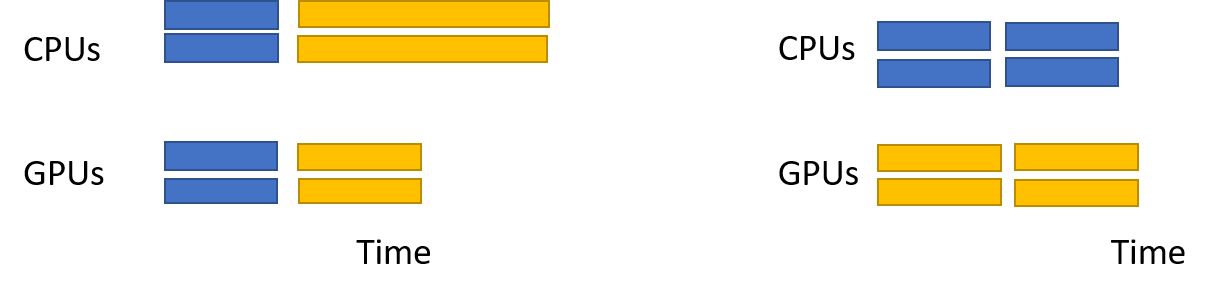
\includegraphics[width=0.8\linewidth]{figs/performance}
% 	\caption{SPT is not necessarily optimal. The ACT for SPT is 15.5 while the act for optimal is  13.5.}
% 	\label{fig:performance}
% \end{figure}

% \subsection{Modeling}

% We model our \name allocation and scheduling problem starting from the workload. In a typical hybrid cluster, assume $C_1,C_2,C_3$ represents the capacity of CPU cores, GPUs and memory from the cluster. there are $n$ active users, and each of them keep submitting machine learning jobs. For each job $j$, when it arrives at time $r_j$, it contains 2 configurations representing the resources demand  
% $$
% 	Q_i=
% 	\begin{bmatrix}
% 	c_i & m_i^1 & p_i^1 \\
% 	g_i & m_i^2 & p_i^2 
% 	\end{bmatrix} $$
% where the first row shows the demand and estimated processing time if the job  will be placed in CPU and the second row show the corresponding GPU configurations.

% Consider the  non-preemptive offline scheduling problem first, the constraints can be formulated as the following:

% \begin{equation}
% \begin{array}{ll@{}ll}
% ~ & \displaystyle\sum\limits_{i,s} x_{i,j,s} =1  & \forall j \\
% ~ &  \displaystyle\sum\limits_{j,s\in (t-p_j^i,t]} x_{i,j,s}c_j \leq   C_1  & ~~\forall i,t \\
% ~ &  \displaystyle\sum\limits_{j,s\in (t-p_j^i,t]} x_{i,j,s}g_j \leq   C_2  & ~~\forall i,t \\
% ~ &  \displaystyle\sum\limits_{j,s\in (t-p_j^i,t]} x_{i,j,s}m_j^i \leq   C_3  & ~~\forall i,t \\
% ~& x_{i,j,s} = 0   & ~~\forall i,j,s > T-p_j^i ~or~s<r_j\\
% & x_{i,j,s} = \{0,1\} & \forall i,j,s\\
% \end{array}
% \end{equation}

% with extra trivial nonnegative constraints. In the above integer programming, $T$ is a trivial upper bound on the makespan of any reasonable schedule. $x_{i,j,s}$ indicates whether job $j$ is processed with computation resource $i$ at starting time $s$. 

% The objective function, depending on ACT or makespan, can be formulated as $\sum\limits_{i,s}x_{i,j,s}(s+p_{j}^i)$ or $\max x_{i,j,s}(s+p_{j}^i)$. However, regardless of what objective we choose, the optimization will be a NP-Hard problem. The hardness come from 2 parts: the multi-dimensional queueing problem, and the rigid job scheduling problem. Hence, for current paper, Our goal is to seek heuristic that works well in the real system.





\subsection{Other challenges}



\desc{Simultaneously improve performance, efficiency, and fairness.}

The tradeoff between performance and fairness is well-known \cite{fairness_efficency_tradeoffs,hug}.
For our problem, if we only optimize for performance using ideas such as shortest job first, users with larger jobs may starve so it is not fair at all.
On the other hand, if we aim at instantaneous fairness such as DRF, there is not much room to improve the performance.
Therefore, the key challenge is how to achieve better job completion time with fairness. 

\desc{Need to estimate the performance of job on CPU or GPU}

On the system side, we need to estimate the job completion times in an online manner with reasonable overhead.
This provides inputs for the scheduler in \name and can free users from setting up the configurations. 


% To achieve the improvement in Figure \ref{fig:motivation_example_2}, we  need to have the estimate of completion times of jobs.
% However, performance prediction is challenging \cite{ernest, cherrypick}.
% First, low accuracy may result in largely negative impact on \name.
% Second, prediction may require large overheads which can make the improvement may not be useful.
% In spite of these challenges, we still want to provide this performance prediction with low overheads and high accuracy.

% It is difficult to optimize performance, efficiency, and fairness simultaneouly.
% If we enforce fair resource allocation among users like Figure \ref{fig:motivation_example_1}, it hurts the performance and efficiency.

% To improve performance, the straight-forward solution is to put the jobs with low speed-up rates on CPUs and jobs with high speed-up rates on GPUs.
% However, it is not true that it also maximizes the efficiency and fairness.
% To demonstrate this, we re-use the motivation example in Table \ref{tbl:mov_example}.
% For instance, we place jobs with large speed-up rates $(\geq 1)$ in GPUs, while putting the small speed-up rates $(<1)$ on CPUs.
% In this case, we actually place all 6 jobs on GPUs but do not use any CPUs that results in low efficiency.

% If we try to optimize the performance and efficiency, it is not trivial to maintain fairness among users.
% When resources are interchangeable, it is actually hard to define fairness.
% Traditional schedulers \cite{yarn, mesos} maintain fairness based on the received resources among users.
% However, this definition of fairness cannot be used when resources are not equally important.
% Naive fair allocation may result in inefficiency like Figure \ref{fig:motivation_example_1}.

% \section{Existing scheduling policies on Yarn}

\desc{Fair Scheduler and Capacity Scheduler in Yarn}

Essentially, Yarn allocates the resources to its active queues. An queue is called active, if there is at least one job. In Yarn, there are two types of schedulers, which are Capacity Scheduler (CS) and Fair Scheduler (FS). Fair Scheduler equally splits cluster resources among the active queues [?]. Meaning, Fair Scheduler pursue the fairness among the queues. In the meantime, Capacity Scheduler is designed to guarantee the resource capacity for each tenant [?]. In addition, There is an added benefit that an organization can access the available resources, which are not used by others. As we bridge the gap that the interactive users are not satisfied with both existing schedulers, we discuss why Fair Scheduler and Capacity Scheduler do not work well on this gap.

\desc{How Fair Scheduler works? Why do we need a new scheduling policy?}

Fair Scheduler organizes the arrival jobs into queue (more precisely, pools), and fairly divides resources between the queues. The queues can be hierarchal in which the same level queues are to receive the same amount of resources. In addition, jobs can be scheduled within a queue. There are 3 fair scheduling policies in Fair Scheduler: First in first out (FIFO), fair, and dominant resource fairness (DRF). 

\begin{itemize}
\item FIFO: FIFO scheduling policy allocates the resource to the coming jobs based on their priorities and arrival times.
\end{itemize}


Fair Scheduler + weight.

Capacity Scheduler.



\section{Online Interchangeable-Resource Allocation Problem}

\subsection{Problem Setting}

\desc{Interchangeability}

In the interchangeable resource allocation problem we considered, there are three resources of interests: CPU, GPU and memory (MEM).
Both CPU and GPU can be used for computational needs in an interchangeable way, MEM demand cannot be replaced by CPU or GPU.
This can be easily extended to include additional resources such as disk I/O, network I/O.

There are $N$ users in the systems. A user has jobs arriving over time.
Job $i$ arrives at time $t_i$, the online profiling tool (\S\ref{sec:res_estimation}) can create 2 configurations estimating the demand and processing time of job $i$ as following: $$
Q_i=
\begin{bmatrix} 
c_i & m_i^1 & p_i^1 \\
g_i & m_i^2 & p_i^2 
\end{bmatrix} $$ where $c_i, m_i^1, p_i^1$ represents the demand for CPU, memory and its estimated processing time from its CPU configuration; $g_i, m_i^2, p_i^2$ represents the demand for GPU, memory and its estimated processing time from its GPU configuration.

Let $C_c, C_g, C_m$ be capacities of CPU cores, GPUs and memory.
$A_c, A_g, A_m$ denotes current loads of the cluster on corresponding resources.

\paragraph{Problem statement} \emph{Given job configurations where jobs can interchange between CPUs and GPUs,
what is the best solution to allocate resources to the jobs such that it maximizes the performance and efficiency while maintains fairness?}

\todo{explain why's it is challenging?}

\subsection{Allocation Policy}

\begin{algorithm}[H]
\small
\caption{\name Online \name Scheduler}
\label{alg:greedy}
\begin{algorithmic}[1]
    \State $C,A:$ System capacity and current load
    \State $L:$ fairness score list of all users
    \State $Queue_i$: all waiting jobs of user $i$ at current time
    \State $U$: user set where the fairness scores of all users in $U$ fall in the lowest $\alpha$\% percentage
    \State $W$: all queueing jobs from set $U$.
    \State $S$: sorted list of all processing times from all jobs in $W$ (sorted increasingly)
    \Procedure{OnlineAlloc()}{}
    \While{$A_c< C_c || A_2 < C_2 ~\&\&~ A_3 < C_3$ }
    \State pick current value $p_n^m$ from list $S$		\Comment{Default is the first value in $S$}
    \If{ $m=2 \&\& A_2+ g_n \leq C_2 ~\&\&~ A_3+m_n^2 \leq C_3$ }  \Comment{GPU config}
    \State{\textsc{JobStart}($L,n$)} 
    \Comment{Place $n$ on GPU}
    \State{Update U,W,S}
    \ElsIf { $m=1 \&\& A_1+ c_n \leq C_1 ~\&\&~ A_3+m_n^1 \leq C_3$ }  \Comment{CPU config}
    \State{\textsc{JobStart}($L,n$)}  \Comment{Place $n$ on CPU}
    \State{Update U,W,S}
    \Else
    \State Move the next job;
    \EndIf
    \EndWhile
    \EndProcedure
    \\
    \Function{JobStart($L,job_j$)}{}  \Comment{Update score if job $j$ starts being processed}
    \State Remove job $j$ from list $W$
    \If {job $j$ is from user $i$}
    \If {$p_j^1 <  p_j^2$} 
    \If {job $j$ is placed on CPU}
    $Value(j) = \max(\frac{c_j}{C_1},\frac{m_j^1}{C_3})$
    \Else ~
    $Value(j) = \frac{p_j^1}{p_j^2}\max(\frac{c_j}{C_1},\frac{m_j^1}{C_3})$
    \EndIf
    \Else
    \If {job $j$ is placed on CPU}
    $Value(j) = \frac{p_j^2}{p_j^1} \max(\frac{g_j}{C_2},\frac{m_j^2}{C_3})$
    \Else ~
    $Value(j) = \max(\frac{g_j}{C_2},\frac{m_j^2}{C_3})$
    \EndIf
    \EndIf
    \EndIf
    \State $L(i) = L(i) + Value(j)$
    \EndFunction     
    \\
    \Function{JobFinish($L,job_j$)}{}  \Comment{Update score if job $j$ finishes}
    \If {job $j$ is from user $i$}
    \State $L(i) = L(i) - Value(j)$
    \EndIf
    \EndFunction
\end{algorithmic}
\end{algorithm}

The allocation policy needs to pack the jobs in the queue across candidate users.
The high level of the policy is as summarized in the following two steps:
(1) Pick a subset of users who receive less than others based on fairness scores.
(2) Schedule jobs of the user subset in to optimize their performance.
The pseudo-code of allocation policy is summarized in Algorithm \ref{alg:greedy}.

To maintain the fairness for step (1), we keep watch on the fairness score of each user.
%As sharing interachanable resources in space domain is not efficient, we need find another way to maintain fairness.
We define the fairness score as \textit{transformed dominant share}.
The idea is the following: Every user wishes his jobs to be finished as fast as possible.
However, that is not doable as some jobs have to sacrifice and take the suboptimal configurations for the performance of other jobs.
The system rewards them for taking a suboptimal solution and finish slower.
Here is how we define \textit{transformed dominant share} value $v(i)$ for a single job $i$. $v(i)$ will be calculated only when it is being processed.
From $$
	Q_i=
	\begin{bmatrix}
	c_i & m_i^1 & p_i^1 \\
	g_i & m_i^2 & p_i^2 
	\end{bmatrix} $$ simply compare $p_i^1$ and $p_i^2$ and check the placement of job $i$. \begin{itemize}
		\item If $p_i^1 <  p_i^2$, and job $i$ is on CPU, then $v(i) = \max(\frac{c_i}{C_1},\frac{m_i^1}{C_3})$.
		\item If $p_i^1 <  p_i^2$, and job $i$ is on GPU, then $v(i) =  (\frac{p_i^1}{p_i^2})^\mu \max(\frac{c_i}{C_1},\frac{m_i^1}{C_3})$.
		\item If $p_i^1 \geq  p_i^2$, and job $i$ is on CPU, then $v(i) =  (\frac{p_i^2}{p_i^1})\mu \max(\frac{g_i}{C_2},\frac{m_i^2}{C_3})$.
		\item If $p_i^1 \geq  p_i^2$, and job $i$ is on GPU, then $v(i) = \max(\frac{g_i}{C_2},\frac{m_i^2}{C_3})$.
	\end{itemize} 
where $\mu \geq 0 $ controls the fairness score when the job is not placed on the preferred resource.
The \textit{transformed dominant share} value of a user is the sum of all values from its jobs that are currently being processed.
\textit{Transformed dominant share} will shrink to DRF if there is only a single configuration.

In step (2), obtaining the optimal schedule is actually a nondeterministic polynomial (NP) time problem. 
We solve this step using heuristic.
A job $i$ has 2 completion times $p^1_i$ and $p^2_i$ on CPU and GPU respectively.
A set with $W$ jobs have $2|W|$ processing times.
We sort the processing times so that we select the job with shortest one to schedule first.
This heuristic is similar to the shortest remaining time first (SRPT) algorithm.

\section{Design Details}
\label{sec:impl}

In this section, we describe how we have implemented \name on Apache YARN, how we use standard techniques for demand estimation, and additional details related to our implementation.

\begin{figure}
\centering
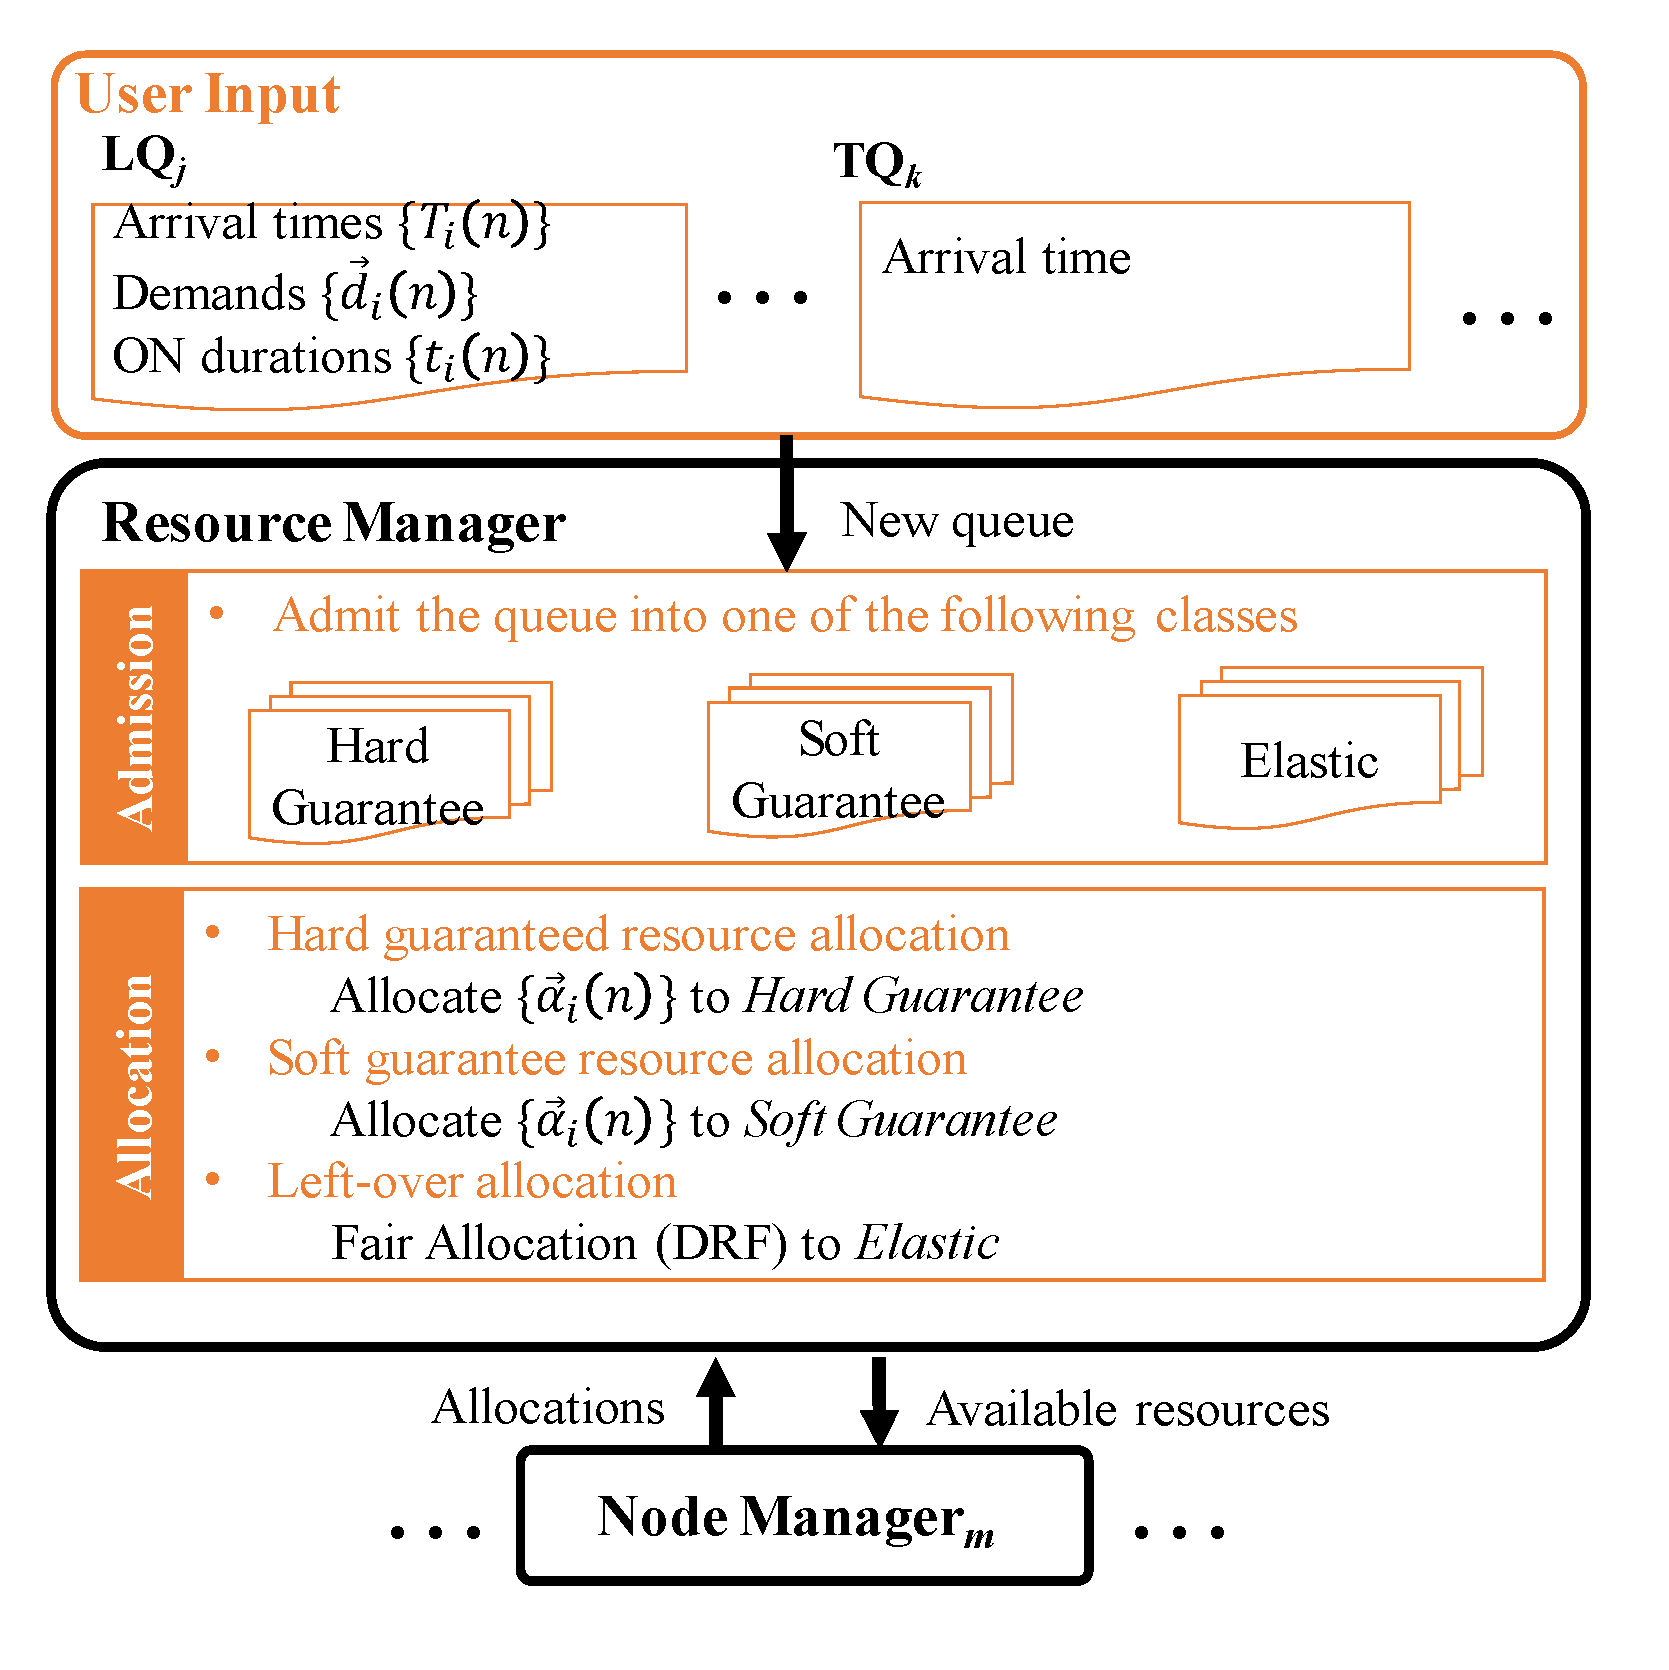
\includegraphics[width=1.0\linewidth]{fig/diagram}
\caption{Enabling bounded prioritization with long-term fairness in a  multi-resource cluster. 
\name-related changes are shown in orange. \todo{change the figure ON durations to deadlines}}
\label{fig:system_design}
\end{figure}

\subsection{Enabling \name in Cluster Managers}
Enabling bounded prioritization with long-term fairness requires implementing the \emph{\name scheduler} itself along with an additional \emph{admission control} module in cluster managers, and it takes \emph{additional information on demand characteristics} from the users. 
A key benefit of {\name} is its simplicity of implementation: we have implemented it in YARN using only $600$ lines of code.
In the following, we describe how and where we have made the necessary changes.

\subsubsection*{Primer on Data-Parallel Cluster Scheduling}
Modern cluster managers typically includes three components: \emph{job manager} or application master (AM), \emph{node manager} (NM), and \emph{resource manager} (RM).

One NM runs on each server in the cluster, and it is responsible for managing resource containers on that server. 
A container is a unit of allocation and are used to run specific tasks. 

For each application, a job manager or AM interacts with the RM to request job demands and receive allocation and progress updates. 
It can run on any server in the cluster. 
AM manages and monitors job demands (memory and CPU) and job status (\texttt{PENDING}, \texttt{IN\_PROGRESS}, or \texttt{FINISHED}). 

The RM is the most important part in terms of scheduling. 
It receives requests from AMs and then schedules resources using an operator-selected scheduling policy. 
It asks NM to prepare resource containers for the various tasks of the submitted jobs.

\subsubsection*{\name Implementation}
We made three changes for taking user input, performing admission control, and calculating resource shares -- all in the RM.
We do not modify NM and AM.
Our implementation also requires more input parameters from the users regarding the demand characteristics of their job queues. 
Figure~\ref{fig:system_design} depicts our design.

\paragraph{User Input} Users submit their jobs to their queues. 
In our system, there are 2 queue types, i.e., {\burstq}s and {\batchq}s. 
We do not need additional parameters for {\batchq}s because they are the same as the conventional queues. 
Hence, we assume that {\batchq}s are already available in the system. 
However, the \name scheduler needs additional parameters for LQs; namely, arrival times and demands.

Users submit a request job that contains their parameters of the new \burstq. 
After receiving the parameters in the job, the RM sets up a new \burstq queue for the user.
Users can also ask the cluster administrator to set up the parameters. 

\paragraph{Admission Control} YARN does not support admission control. 
We implement an admission control module to classify {\burstq}s and {\batchq}s into Hard Guarantee, Soft Guarantee, and Elastic classes. 
A new queue is rejected if it cannot meet the safety condition \eqref{eqn:ad-safety}, which invalids the committed performance.
If it is a \batchq, it is added into the Elastic class.
If the new {\burstq} does not satisfy the fairness condition \eqref{eqn:ad-fair}, it is also admitted to the Elastic class.
If the new {\burstq} meets the fairness condition \eqref{eqn:ad-fair}, but fails at the resource condition \eqref{eqn:ad-enough}, it will be put in the Soft Guarantee class.
If the new {\burstq} meets all the three conditions, i.e., safety, fairness, and resource, it will be admitted to the Hard Guarantee class.

\paragraph{\name Scheduler} We implement \name as a new scheduling policy to achieve our joint goals of bounded priority with long-term fairness. 
Upon registering the queues, users submit their jobs to their {\burstq}s or {\batchq}s. 
Thanks to admission control, {\burstq}s and {\batchq}s are classified into Hard Guarantee, Soft Guarantee, and Elastic classes. 
Note that resource sharing policies are implemented across queues in YARN, jobs in the same queue are scheduled in FIFO manner.
Hence, \name only sets the share at the individual queue level.

\name Scheduler periodically set the share levels to all {\burstq}s in Hard Guarantee and Soft Guarantee classes.
These share levels are actually upper-bounds on resource allocation that an {\burstq} can receive from the cluster. 
Based on the real demand of each {\burstq}, \name allocates resources until it meets the share levels\delete{ (whether it is in the ON period or OFF period)}. 

\name Scheduler allocates the resource to the three classes in the following priority order: (1) Hard Guarantee class, (2) Soft Guarantee class, and (3) Elastic class. 
The {\burstq}s in the Hard Guarantee class are allocated first.
Then, the \name continues allocates the resource to the {\burstq}s in Soft Guarantee class.
The queues in the Elastic class are allocated with left-over resources using DRF \cite{drf}.

%To ensure work conservation, unused resources by all queues are combined and redistributed across queues in the Elastic class using DRF \cite{drf}. 

\subsection{Demand Estimation}

\name requires accurate estimates of resource demands and their durations of \burstq jobs by users. 
These estimations can be done by using well-known techniques; \eg, users can use history of prior runs \cite{rope, jockey, tetris} with the assumption that resource requirements for the tasks in the same stage are similar \cite{drf, pacman, paratimer}. 
We do not make any new contributions on demand estimation in this paper. 
%While {\name} performs the best with accurate estimations, we have found that {\name} is robust to small misestimations in practice (\S\ref{sec:performance_large_scale}).
When LQs have bursty arrivals of different sizes, BPF with the $\alpha$-strategy ensures the performance with the average usage remains similar (\S\ref{sec:performance_large_scale}). 
We consider a more thorough study an important future work. 

\subsection{Operational Issues}

\paragraph{Container Reuse}
Container reuse is a well-known technique that is used in some application frameworks, such as Apache Tez. 
The objective of container reuse is to reduce the overheads of allocating and releasing containers. 
The downside is that it causes resource waste if the container to be reused is larger than the real demand of the new task. 
Furthermore, container reuse is not possible if the new task requires more resource than existing containers. 
For our implementation and deployment, we do not enable container reuse because {\name} periodically prefers more free resources for \burstq jobs, causing its drawbacks to outweigh its benefits in many cases.

\paragraph{Preemption}
Preemption is a recently introduced setting in the YARN Fair Scheduler \cite{hadoop-fair-scheduler}, and it is used to kill running containers of one job to create free containers for another. 
By default, preemption is not enabled in YARN. 
For {\name}, using preemption can help in providing guarantees for {\burstq}s. 
However, killing the tasks of running jobs often results in failures and significant delays. 
We do not use preemption in our system throughout this paper.

%\subsection{Possible issues}

%In the same worker node, containers are sequentially launched. Slow allocation of containers may hurt resource guarantee.

% % old text % %
%\begin{algorithm}
%\caption{Scheduler}
%\label{algorithm1}
%\begin{algorithmic}[1]
%\Procedure{periodicSchedule()}{}
%\State $\{\mathbb{A}, \mathbb{B}, \mathbb{U}\}$ = \textsc{updateQueueStatus}($\mathbb{A}$,$\mathbb{B}$,$\mathbb{U}$)
%\If{\textsc{isNewArrival}($\mathbb{Q}$)}
%	\State Update the best effort queues: $\mathbb{U} = \mathbb{U} \cup \mathbb{Q}$
%\EndIf
%\State $\{\mathbb{A}, \mathbb{B}, \mathbb{U}\}$ = \textsc{admit}($\mathbb{U}$)
%\State \textsc{allocate}($\mathbb{A}$,$\mathbb{B}$)
%\State Obtain the available cluster resources $\myvec{L}$
%\State DRF($\mathbb{U}$, $\myvec{L}$)
%\EndProcedure
%\\
%\Function{updateQueueStatus($\mathbb{A}$,$\mathbb{B}$,$\mathbb{U}$)}{}
%\ForAll{queue $A \in \mathbb{A}$}
%	\If{queue $A$ is deactivated}  Update $\mathbb{A} = \mathbb{A} \setminus A$
%	\EndIf
%\EndFor
%\ForAll{queue $B \in \mathbb{B}$}
%	\If{queue $B$ is deactivated} Update $\mathbb{B} = \mathbb{B} \setminus B$
%	\EndIf	
%\EndFor
%\ForAll{queue $U \in \mathbb{U}$}
%	\If{queue $U$ is deactivated} Update $\mathbb{U} = \mathbb{U} \setminus U$
%	\EndIf
%\EndFor
%\State \textbf{return} $\{\mathbb{A} , \mathbb{B},\mathbb{U}  \}$	
%\EndFunction
%\\
%\Function{admit(queues $\mathbb{U}$)}{}
%\ForAll{queue $U \in \mathbb{U}$}
%	\If{queue $U$ is a bursty queue}
%		\If{admission conditions \eqref{eqn:bursty_adm_cond_2} satisfied}
%			\State Update $\mathbb{A} = \mathbb{A} \cup U$
%			\State Update $\mathbb{U} = \mathbb{U} \setminus U$
%		\EndIf
%	\Else
%		\If{admission condition \eqref{eqn:batch_adm_cond} satisfied}
%			\State Update $\mathbb{B} = \mathbb{B} \cup U$
%			\State Update $\mathbb{U} = \mathbb{U} \setminus U$
%		\EndIf
%	\EndIf
%\EndFor
%\State \textbf{return} $\{\mathbb{A} , \mathbb{B},\mathbb{U}  \}$	
%\EndFunction
%\\
%\Function{\diff{allocate}($\mathbb{A}$, $\mathbb{B}$)}{}
%\ForAll{bursty queue $A \in \mathbb{A}$}
%		\State Compute $\myvec{a_i}$ allocated to queue $A$ as \eqref{eqn:alpha_1}, \eqref{eqn:alpha_2a}
%\EndFor
%\State Obtain the available cluster resources $\myvec{L}$
%\State $\myvec{R_b}$ = \textsc{DRF}($\mathbb{B}$,$\myvec{L}$) as Algorithm 1 of \cite{drf}.  
%\EndFunction
%\end{algorithmic}
%\end{algorithm}


\section{Evaluation}

\paragraph{Setup.} We use the real-trace workloads from Google.

\emph{Workload}

\emph{Experimental setup}

\emph{Simulation setup}

\paragraph{Metrics}

\subsection{Experimental Results}

\subsubsection{Performance Guarantee}

\subsubsection{Long-term Fairness}

\subsection{Simulations}

\subsection{\name in Testbed Experiments}
\label{sec:testbed}

\subsubsection{BPF in practice}

\begin{figure}[!t]
    \centering
    
\includegraphics[width=0.3\linewidth]{fig/b1_mov_legend} 
    \\
    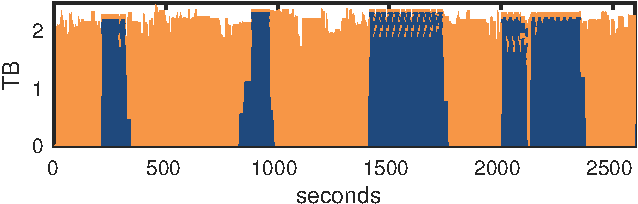
\includegraphics[width=0.8\linewidth]{fig/b1_mov_SpeedFair_BB} 
    \caption{[Cluster] \name's solution for the motivational problem (\S\ref{sec:ex}). The first two jobs of {\burstq} quickly finish and the last two jobs are prevented from using too much resource. This solution is close to the optimal one.}
    \label{fig:solution}
\end{figure}

Before diving into the details of our evaluation, recall the motivational problem from Section~\ref{sec:ex}. 
Figure~\ref{fig:solution} depicts how \name solves it in the testbed. \name enables the first two jobs of {\burstq} to quickly finish in 141 and 180 seconds.
For the two large jobs arriving at 1400 and 2000 seconds, the share is very large only in roughly 335 seconds but it is cut down to give back resource to {\batchq}.
%The large job arrives at 1400 seconds is not continuously allocated with large resources like SP.

\subsubsection{Performance guarantee}
\label{sec:performane_guarantee}

\begin{figure}[!t]
\centering
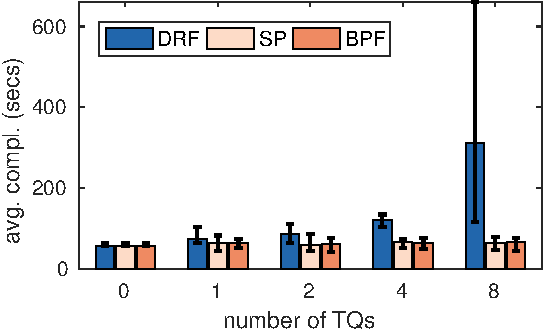
\includegraphics[width=0.8\linewidth]{fig/busty_perf_grt_err_BB}
\caption{[Cluster] Average completion time of \burstq jobs in a single \burstq across the 3 schedulers when varying the number of {\batchq}s. \name and SP guarantee the average completion time of the \burstq jobs while DRF significantly suffers from the increase of number of {\batchq}s.}
\label{fig:busty_perf_grt}
\end{figure}
 
Next, we focus on what happens when there are more than one \batchq.
Figure \ref{fig:busty_perf_grt} shows that average completion time of \burstq jobs in the 40-node cluster on the BB workload. In this setting, there are a single \burstq and multiple {\batchq}s. The x-axis shows the number of TQs in the cluster.

When there are no TQs, the average completion times of \burstq jobs across three schedulers are the same (57 seconds).
The completion times are greater than the average ON period (27 seconds) because of inefficient resource packing and allocation overheads.
In practice, the resource demand of tasks cannot utilize all resources of a node that results in large unallocated resources across multiple nodes.
Hence, the \burstq jobs are not able to receive the whole cluster capacity as expected.
More importantly, this delay is also caused by allocation overheads, such as waiting for containers to be allocated or launching containers.

As the number of {\batchq}s increases, the performance of DRF significantly degrades because DRF tends to allocate less resource to {\burstq} jobs.
DRF is the worst among three schedulers. In contrast, \name and SP give the highest priority to {\burstq}s that guarantees the performance of \burstq jobs.
The average completion times, when TQs are available (1,2,4, and 8), are almost the same (65 seconds).
These average completion times are still larger than the case of no TQs because of non-preemption.
The \burstq jobs are not able to receive the resources that are still used by the running tasks. 

\begin{table}[!t]
\centering
\caption{[Cluster] Factor of improvement by \name across various workload with respect to the number of {\batchq}s.} 
\begin{tabular}{|c|c|c|c|c|} \hline
\small
\centering
Workload & 1 TQ  & 2 TQs & 4 TQs & 8 TQs \\ \hline \hline
BB & 1.18 & 1.42 & 1.86 & 4.66 \\ \hline 
TPC-DS &  1.35 &   1.61  &  2.29  &  5.38  \\ \hline 
TPC-H & 1.10  & 1.37 & 2.01 &  5.12\\ \hline 
\end{tabular}
\label{tbl:speed_up}
\end{table}

To understand how well \name performs on various workload traces, we carried out the same experiments on TPC-DS and TPC-H.
As SP and \name achieve the similar performance, we only present the factors of improvement of \name across the various workloads in Table \ref{tbl:speed_up}.
The numbers on the table show the consistent improvement on the average completion time of \burstq jobs. 

\begin{figure}[!t]
    \centering
    \subfloat[1 LQ \& 4 TQs]{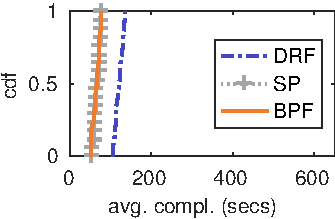
\includegraphics[width=0.48\linewidth]{fig/busty_perf_grt_cdf4_BB} \label{fig:busty_perf_grt_cdf_a}}    
    \subfloat[1 LQ \& 8 TQs]{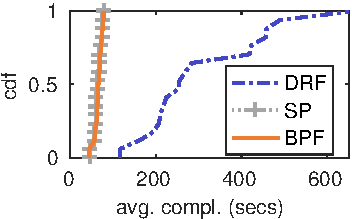
\includegraphics[width=0.48\linewidth]{fig/busty_perf_grt_cdf8_BB} \label{fig:busty_perf_grt_cdf_b}}
    \caption{[Cluster] The completion time of LQ jobs is predictable using \name.}
    \label{fig:busty_perf_grt_cdf}
    \vspace{-0.4cm}
\end{figure}

In addition to the average completion time, we evaluated the performance of individual \burstq jobs.
Figure \ref{fig:busty_perf_grt_cdf} shows that cumulative distribution functions (cdf) of the completion times across 3 approaches.
Figure \ref{fig:busty_perf_grt_cdf_a} and \ref{fig:busty_perf_grt_cdf_b} are the experimental results for the cases of 4 {\batchq}s and 8 {\batchq}s, respectively.
We observe that the completion times of \burstq jobs in DRF are not stable and vary a lot when the number of {\burstq}s becomes large as in Figure \ref{fig:busty_perf_grt_cdf_b}.
The unstable performance is caused by the instantaneous fairness and the variance of total resource demand.

\subsubsection{Fairness guarantee}
\label{sec:fairness_guarantee}

\begin{figure}[!t]
    \centering
    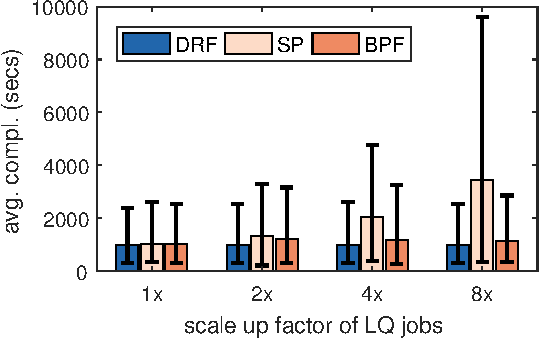
\includegraphics[width=0.8\linewidth]{fig/batch_perf_protect_BB} 
%    \\
%    \subfloat[LQ jobs]{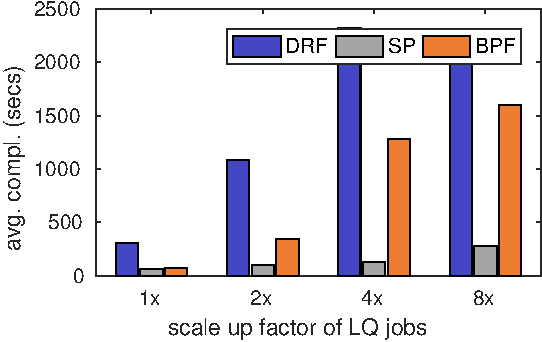
\includegraphics[width=1\linewidth]{fig/long_busty_BB} \label{fig:protecting_batch_jobs_b}}
    \caption{[Cluster] \name protects the batch jobs up to $3.05\times$ compared to SP.}
    \vspace{-0.3cm}
    \label{fig:protecting_batch_jobs}
\end{figure}

Figure \ref{fig:protecting_batch_jobs} shows the average completion time of \batchq jobs when we scale up the number of tasks of \burstq jobs are by 1x, 2x, 4x, and 8x.
In this experiment, there are a single \burstq and 8 {\batchq}s.

Since DRF is a fair scheduler, the average completion times of \batchq jobs are almost not affected by the size of \burstq jobs.
However, SP allocates too much resource to \burstq jobs that significantly hurts \batchq jobs.
Since SP provides the highest priority for the {\burstq} jobs, it makes the {\batchq} jobs to starve for resources.
\name performs closely to DRF.
While DRF maintains instantaneous fairness, \name maintains the long-term fairness among the queues.


%\begin{figure}[!t]
%\centering
%    {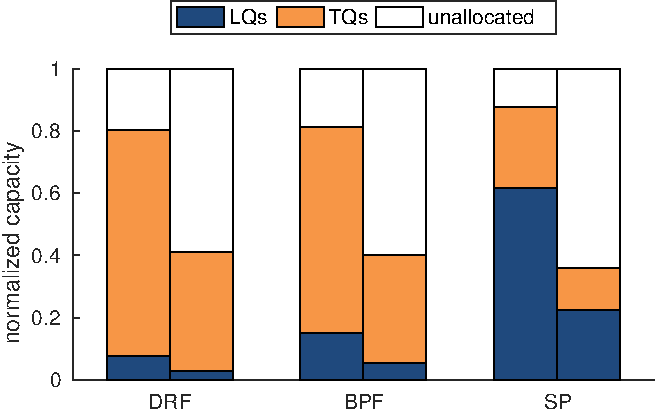
\includegraphics[width=0.8\linewidth]{fig/b8_avg_res_BB}}
%\caption{[Cluster] The average resource consumption of the cases of scaling up \burstq jobs at 8x. The left bar is memory usage, and the right bar is CPU usage. All three policies have similar utilization.}
%\label{fig:avg_res}
%\end{figure}

%To better see the long-term fairness in resource allocation, we present average resource usage across 3 approaches in Figure \ref{fig:avg_res}.
%There are totally 9 queues (1 \burstq and 8 \batchq). The x-axis is the normalized capacity.
%SP is dominant in both memory and CPU.
%\name and DRF can achieve the fairness in resource allocation for {\burstq}s and {\batchq}s.
%All of them have similar resource utilization.

\subsubsection{Scheduling overheads}

Recall from Section \ref{sec:impl} that the \name scheduler has three components: user input, admission control, and allocation.
Compared to the default schedulers in YARN, our scheduler has additional scheduling overheads for admission control and additional computation in allocation.

Since we only implement our scheduler in the Resource Manager, the scheduling overheads occur at the master node.
To measure the scheduling overheads, we run admission control for 10000 \burstq queues and 10000 \batchq queues on a master node -- Intel Xeon E3 2.4 GHz (with 12 cores).
Each LQ queue has 500 ON/OFF cycles.
Recall the \textsc{LQAdmit} and \textsc{TQAdmit} functions in Algorithm \ref{algorithm1}, the admission overheads increase linearly to the number of queues.
The total admission overheads are approximately 1 ms, which is much less than the default update interval in YARN Fair Scheduler, i.e., 500 ms \cite{hadoop-fair-scheduler}.
The additional computation in allocation is also negligibly less than 1 ms.

%\begin{table*}
%\centering
%\caption{Scheduling overheads} 
%\begin{tabular}{|c|p{10cm}|c|} \hline
%Type & Description & Avg. Time \\ \hline \hline
%Job submission & Job is submitted from client to YARN & 13.22 secs \\ \hline
%Container allocation & YARN localizes and allocates a container for a task.  &  0.04 secs \\ \hline
%Task setup & Tez setup a task to run on the allocated container. & 6.24 secs \\ \hline
%Launching Tez task & Launching a Tez task on the container & 1.17 secs \\ \hline
%Task stop & Tez stops the container use on a finished task. & 0.21 secs\\ \hline
%Container release & YARN releases the running container. & 5.19 secs \\ \hline
%\end{tabular}
%\label{tbl:schedulingOverheads}
%\end{table*}

\subsubsection{Admission control for multiple LQs}
\label{sec:admission}

\begin{figure}[!h]
	\centering
	
\includegraphics[width=0.6\linewidth]{fig/b1i3_res_usage_legend} 
	\vspace{-0.1cm}
	\subfloat[DRF: \burstq-0, \burstq-1, \burstq-2 are unhappy with high latency.]{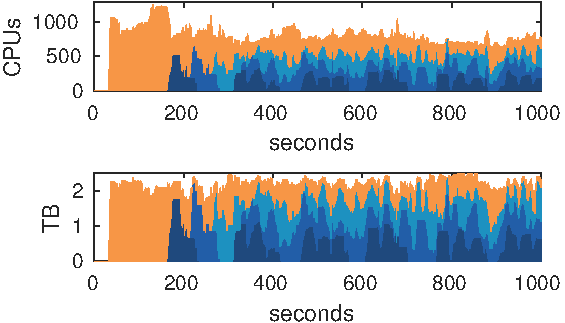
\includegraphics[width=0.8\linewidth]{fig/res_usage_b1i3_DRF_BB} \label{fig:admission_drf_cluster}} 

	\subfloat[SP: \batchq-0 is starving of resources.]{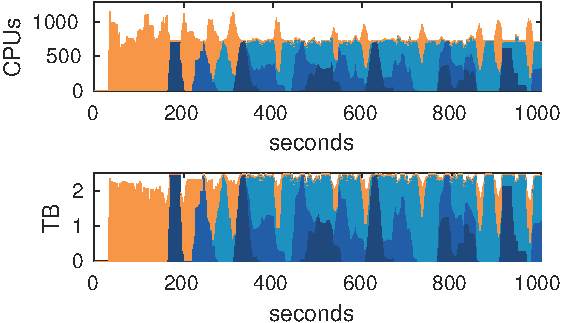
\includegraphics[width=0.8\linewidth]{fig/res_usage_b1i3_SP_BB} \label{fig:admission_strict_cluster}}
    
	\subfloat[N-\name: Only {\burstq}-0 and {\batchq}-0 are happy.]{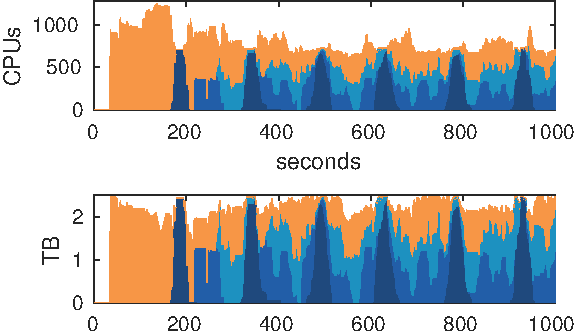
\includegraphics[width=0.8\linewidth]{fig/res_usage_b1i3_N-BPF_BB} \label{fig:admission_hard_cluster}}
   
	\subfloat[\name: {\burstq}-0, {\burstq}-1 and {\batchq}-1 are happy.]{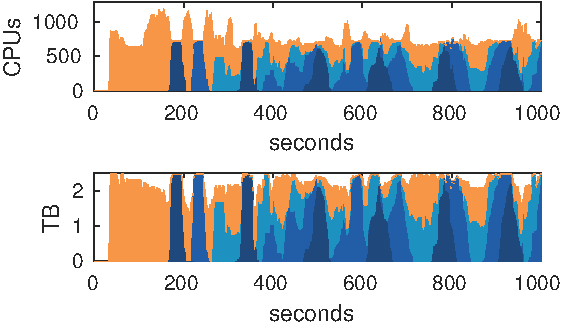
\includegraphics[width=0.8\linewidth]{fig/res_usage_b1i3_BPF_BB} \label{fig:admission_speedfair_cluster}}

	\caption{[Cluster]. DRF and SP fail to guarantee both performance and fairness simultaneously. \name gives the best performance to \burstq-0, near optimal performance for \burstq-1, and maintains fairness among 4 queues. \burstq-2 requires too much resource, so its performance cannot be guaranteed.}
	\label{fig:admission_control_cluster}
\end{figure}


To demonstrate how \name works with multiple {\burstq}s, we set up 3 {\burstq}s (\burstq-0, \burstq-1, and \burstq-2) and a single \batchq (TQ-0).
The jobs \batchq-0 are queued up at the beginning while \burstq-0, \burstq-1, and \burstq-2 arrive at 50, 100, and 150 seconds, respectively.
The periods of {\burstq}-0, {\burstq}-1, and {\burstq}-2 are 150, 110, and 60 secs. All the {\burstq}s jobs have the identical demand and task durations.
The TQ jobs are chosen from the BB benchmark.
\name admits {\burstq}-0 to the Hard Guarantee class, {\burstq}-1 to the Soft Guarantee class, and {\burstq}-2 to the Elastic class.

Figure \ref{fig:admission_drf_cluster} shows the resource usage (CPU and memory) for each queue across four schedulers, i.e., DRF, SP, N-\name and \name.
As an instantaneously fair scheduler, DRF continuously maintains the fair share for all queues as in Figure \ref{fig:admission_drf_cluster}.
Since \burstq-2 requires a lot of resources, SP makes \batchq-0 starving for resources (Figure \ref{fig:admission_strict_cluster}). N-\name provides \burstq-0 with resource guarantee and it fairly share the resources to \burstq-1, \burstq-2, and \batchq-0 (Figure \ref{fig:admission_hard_cluster}).
\name provides hard guarantee to \burstq-0 and soft guarantee to \burstq-1 as in Figure \ref{fig:admission_speedfair_cluster}.
The soft guarantee allows \burstq-1 performs better than using N-\name.
Since \burstq-2 demands too much resources, \name treats it like \batchq-0.

Figure \ref{fig:avg_multi_queue_cluster} shows the average completion time of jobs on each queue across the four schedulers.
The performance of DRF for \burstq jobs is the worst among the four schedulers but it is the best for only \batchq-0.
The performance of SP is good for \burstq jobs but it is the worst for \batchq jobs.
N-\name provides the best performance for \burstq-0 but not \burstq-1 and \burstq-2.
\name is the best among the four schedulers.
The three of four queues, i.e., \burstq-0, \burstq-1, and \batchq-0, significantly benefit from \name.
\name even outperforms SP for \burstq-0 and \burstq-1 jobs and does not hurt any {\batchq}.

\begin{figure}[!h]
	\centering
	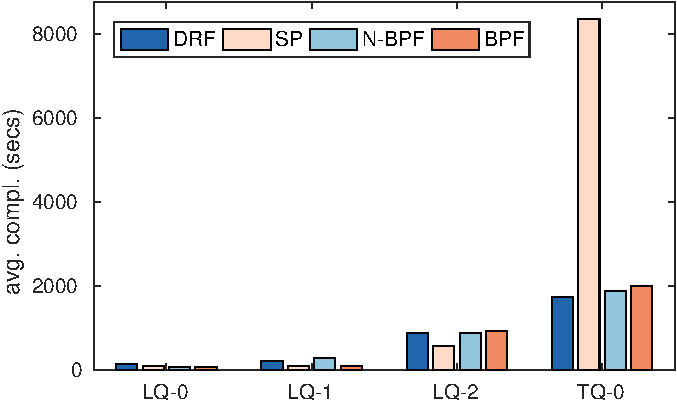
\includegraphics[width=0.8\linewidth]{fig/avg_multi_queues_impl}
	\caption{[Cluster] \name provides with better performance for {\burstq}s than DRF and N-\name. Unlike SP, \name protects the performance of \batchq jobs.}
	\label{fig:avg_multi_queue_cluster}
\end{figure}


\subsection{Performance in Trace-Driven Simulations}
\label{sec:performance_large_scale}

%\subsubsection{Benchmarks' performance in simulations}

To verify the correctness of the large-scale simulator, we replayed the BB trace logs from cluster experiments in the simulator.
Table \ref{tbl:speed_up_sim} shows the factors of improvement in completion times of \burstq jobs for BB workload in simulation that are consistent with that from our cluster experiments (Table \ref{tbl:speed_up}). 

\begin{table}[!t]
\small
\centering
\begin{tabular}{|c|c|c|c|c|c|c|} \hline
\multirow{2}{*}{Workload} &  \multicolumn{5}{c}{Number of {\batchq}s} & \\ \hhline{~------}
 & 1 & 2 & 4 & 8 & 16 & 32 \\ \hline \hline
BB & 1.08  & 1.56 & 2.32 & 4.09 & 7.28 & 16.61  \\ \hline 
TPC-DS & 1.06 & 1.38 & 1.66 & 2.93 & 5.16 & 10.40 \\ \hline 
TPC-H  & 1.01 & 1.28 & 1.92 & 3.04 & 5.50 & 11.35 \\ \hline 
\end{tabular}
\caption{[Simulation] Factors of improvement by \name across various workloads w.r.t the number of {\batchq}s.} 
\label{tbl:speed_up_sim}
\end{table}

\name significantly improves over DRF when we have more {\batchq}s.
We note that the factors of improvement for TPC-DS and TPC-H in the simulation are less that of the cluster experiments.
It turns out that DRF in TCP-DS and TPC-H suffers from the allocation overheads that our simulation does not capture.
The allocation overheads for the \burstq jobs in TPC-DS and TPC-H are large because they have more phases than the \burstq jobs in BB (only 2 phases).

%\subsubsection{Admission control for Multiple LQs}
\label{sec:admission_sim}

\begin{figure}[!h]
    \centering
    
\includegraphics[width=0.8\linewidth]{fig/res_usage_b1i3_legend} 
    \vspace{-0.2cm}
    \subfloat[DRF: \burstq-0, \burstq-1, \burstq-2 are unhappy with high latency.]{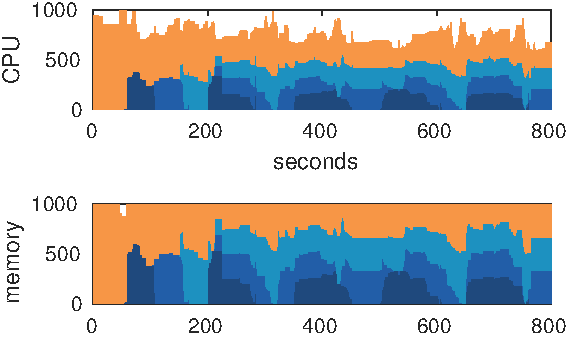
\includegraphics[width=0.8\linewidth]{fig/b1i3_res_usage_drf} \label{fig:admission_drf}} 
    \vspace{-0.1cm}
    \subfloat[SP: \batchq-0 is starving of resources.]{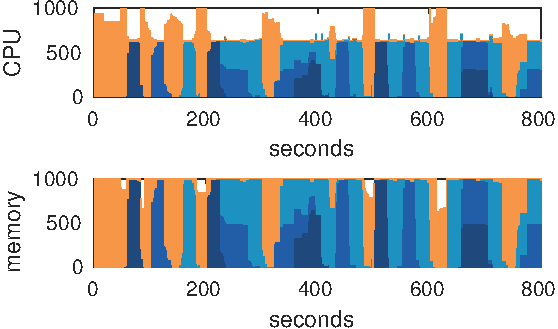
\includegraphics[width=0.8\linewidth]{fig/b1i3_res_usage_strict} \label{fig:admission_strict}}
    \vspace{-0.1cm}            
    \subfloat[N-\name: Only {\burstq}-0 and {\batchq}-0 are happy.]{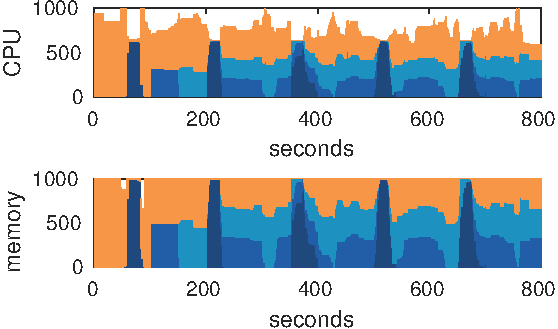
\includegraphics[width=0.8\linewidth]{fig/b1i3_res_usage_Hard} \label{fig:admission_hard}}
    \vspace{-0.1cm}    
    \subfloat[\name: {\burstq}-0, {\burstq}-1 and {\batchq}-1 are happy.]{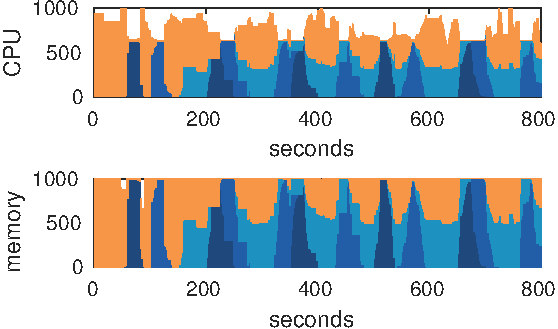
\includegraphics[width=0.8\linewidth]{fig/b1i3_res_usage_speedfair} \label{fig:admission_speedfair}}
    \vspace{-0.1cm}    
    \caption{[Simulation] DRF and SP fail to guarantee both performance and fairness simultaneously. \name gives the best performance to \burstq-0, near optimal performance for \burstq-1, and maintains fairness among 4 queues. \burstq-2 requires too much resource, so its performance cannot be guaranteed.}
    \vspace{-0.5cm}    
    \label{fig:admission_control}
\end{figure}


To demonstrate how \name works with multiple {\burstq}s, we set up 3 {\burstq}s (\burstq-0, \burstq-1, and \burstq-2) and a single \batchq (TQ-0).
The jobs \batchq-0 are queued up at the beginning while \burstq-0, \burstq-1, and \burstq-2 arrive at 50, 100, and 150 seconds, respectively.
The periods of {\burstq}-0, {\burstq}-1, and {\burstq}-2 are 150, \diff{110}, and 60 secs. All the {\burstq}s jobs have the identical demand and task durations.
The TQ jobs are chosen from the BB benchmark.
\name admits {\burstq}-0 to the Hard Guarantee class, {\burstq}-1 to the Soft Guarantee class, and {\burstq}-2 to the Elastic class.

Figure \ref{fig:admission_control} shows the resource usage (CPU and memory) for each queue across four schedulers, i.e., DRF, SP, N-\name and \name.
The capacity of CPU or memory is 1000 nodes.
As an instantaneously fair scheduler, DRF continuously maintains the fair share for all queues as in Figure \ref{fig:admission_drf}.
Since \burstq-2 requires a lot of resources, SP makes \batchq-0 starving for resources (Figure \ref{fig:admission_strict}). N-\name provides \burstq-0 with resource guarantee and it fairly share the resources to \burstq-1, \burstq-2, and \batchq-0 (Figure \ref{fig:admission_hard}).
\name provides hard guarantee to \burstq-0 and soft guarantee to \burstq-1 as in Figure \ref{fig:admission_speedfair}.
The soft guarantee allows \burstq-1 performs better than using N-\name.
Since \burstq-2 demands too much resources, \name treats it like \batchq-0.

Figure \ref{fig:avg_multi_queue} shows the average completion time of jobs on each queue across the four schedulers.
The performance of DRF for \burstq jobs is the worst among the four schedulers but it is the best for only \batchq-0.
The performance of SP is good for \burstq jobs but it is the worst for \batchq jobs.
N-\name provides the best performance for \burstq-0 but not \burstq-1 and \burstq-2.
\name is the best among the four schedulers.
The three of four queues, i.e., \burstq-0, \burstq-1, and \batchq-0, significantly benefit from \name.
\name even outperforms SP for \burstq-0 and \burstq-1 jobs and does not hurt any {\batchq}.

\begin{figure}[!h]
    \centering
    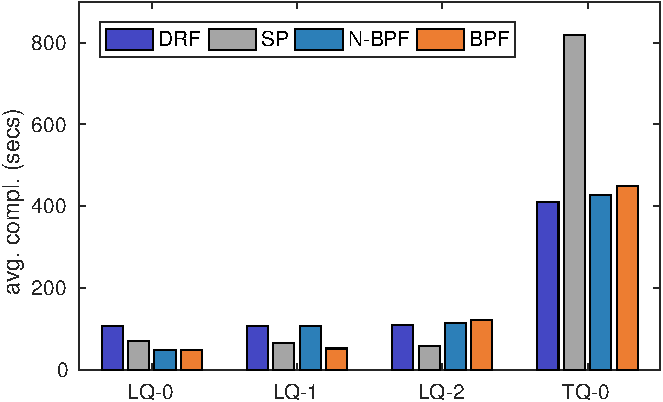
\includegraphics[width=0.8\linewidth]{fig/avg_multi_queuesadmit}
    \caption{[Simulation] \name provides with better performance for {\burstq}s than DRF and N-\name. Unlike SP, \name protects the performance of \batchq jobs.}
    \label{fig:avg_multi_queue}
\end{figure}


%\subsection{Sensitivity Analysis}
%\label{sec:sensitivity_analysis}
%
We use the large-scale simulator to study the impact of estimation errors and non-preemption on \burstq jobs. 
In both cases, \name still outperforms DRF significantly. Results are omitted due to space limit.
%
%\subsubsection{Impact of estimation errors}
%\label{sec:estimation_error_sim}
%
%\name requires users to report their estimated demand for \burstq jobs.
%However, it is challenging to estimate the demand accurately, which naturally results in estimation errors.
%To understand the impact of estimation errors on \name, we assume that estimation errors $e(\%)$ follow the standard normal distribution with zero mean.
%The standard deviation (std.) of estimation errors lines in $[0, 50]$.
%To adopt the estimation errors, we update the task demand and durations of \burstq jobs as $ {task}_{new} = {task}_{original}*(1+e/100)$.
%
%Figure \ref{fig:sen_analysis_est_err} shows the impact of estimation errors on the average completion time of \burstq jobs.
%There are 1 single \burstq and 8 {\batchq}s.
%\burstq jobs arrive every 350 seconds.
%\name is robust when the standard deviation of estimation errors vary 0 to 20.
%The \burstq jobs in BB suffer more from the large estimation errors (std. $>30$) than that of TPC-DS and TPC-H.
%The delays are caused by the underestimated jobs because the excessive demand is not guaranteed by the system.
%Meanwhile, the overestimated jobs do not suffer any delays as the guaranteed resource is more than needed.
%Although estimation errors result in performance degradation, the performance of \burstq jobs is still much better than that of DRF (162 seconds).
%%In the case of large errors, users are suggested reporting larger demands and longer stage-1 durations to improve the performance.\todo{Sentence doesn't parse.}
%
%\begin{figure}[!h]
%\centering
%    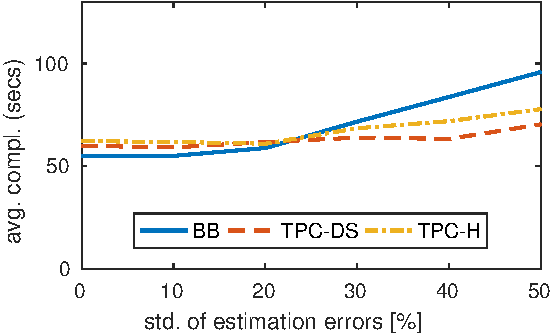
\includegraphics[width=0.7\linewidth]{fig/sen_analysis_est_err}
%\caption{[Simulation] \name's performance degrades with larger estimation errors, yet is still significantly better than DRF (162 secs).}
%\label{fig:sen_analysis_est_err}
%\end{figure}
%
%
%\subsubsection{Impact of non-preemption}
%\label{sec:non_preemption_sim}
%
%To evaluate the impact of non-preemption, we vary the average task durations of {\batchq} jobs.
%The longer task duration is, the longer the task holds its resources.
%In this evaluation, we set up 1 \burstq and 8 {\batchq}s on the simulator.
%Each \burstq job arrives every 350 secs.
%The evaluation is run on three workloads BB, TPC-DS, and TPC-H.
%
%\begin{figure}[!h]
%\centering
%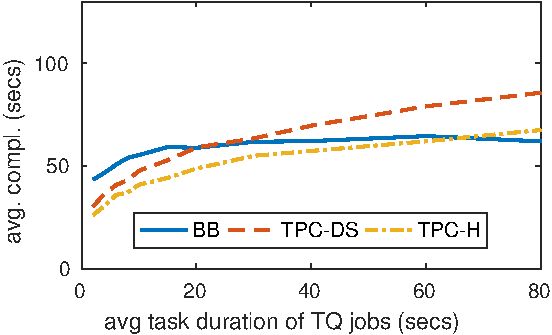
\includegraphics[width=0.7\linewidth]{fig/sen_analysis_task_duration}
%\caption{[Simulation] With longer average task durations, the impact of non-preemption on the performance of \burstq jobs becomes larger. However, the average completion time is still significantly better than that of DRF (162 secs).}
%\label{fig:sen_analysis_task_duration}
%\end{figure}
%
%Figure \ref{fig:sen_analysis_task_duration} shows the impact of average task durations of \batchq jobs on the average completion time of \burstq jobs.
%When we increase the average task durations, the performance of \burstq jobs is degraded.
%Due to the variations of task durations, the BB curve stops increasing from 20, while the TPC-DS and TPC-H curves keep going up.
%Recall the distributions of the task durations in Figure \ref{fig:worklad_cdf}: 70 percent of tasks in BB are very short.
%When the average task durations are more than 20 seconds, there are still a large number of short tasks in BB that allows \name to allocate more resources to \burstq jobs.
%TPC-DS and TPC-H have more variations of task durations that result in increasing delay for \burstq jobs.





\section{Related Work}
\label{sec:related}

\paragraph{Bursty Applications in Big Data Clusters}
Big data clusters experience burstiness from a variety of sources, including periodic jobs \cite{jockey, rope, scarlett, omega}, interactive user sessions \cite{splunk-analysis}, as well as streaming applications \cite{spark-streaming, millwheel, trident}. 
Some of them show predictability in terms of inter-arrival times between successive jobs (\eg, Spark Streaming \cite{spark-streaming} runs periodic mini batches in regular intervals), while some others follow different arrival processes (\eg, user interactions with large datasets \cite{splunk-analysis}).
Similarly, resource requirements of the successive jobs can sometimes be predictable, but often it can be difficult to predict due to external load variations (\eg, time-of-day or similar patterns); the latter, without {\name}, can inadvertently hurt batch queues (\S\ref{sec:motivation}). 

\paragraph{Multi-Resource Job Schedulers}
Although early jobs schedulers dealt with a single resource \cite{late, mantri, quincy}, modern cluster resource managers, \eg, Mesos \cite{mesos}, YARN \cite{yarn}, and others \cite{omega, borg, cosmos}, employ multi-resource schedulers \cite{drf, sjf, tetris, carbyne, apollo, mercury, hdrf} to handle multiple resources and optimize diverse objectives. 
These objectives can be fairness (\eg, DRF \cite{drf}), performance (\eg, shortest-job-first (SJF) \cite{sjf}), efficiency (\eg, Tetris \cite{tetris}), or different combinations of the three (\eg, Carbyne \cite{carbyne}).
% 
However, \emph{all} of these focus on instantaneous objectives, with instantaneous fairness being the most common goal. 
To the best of our knowledge, {\name} is the first multi-resource job scheduler with long-term memory.

\paragraph{Handling Burstiness}
Supporting multiple classes of traffic is a classic networking problem that, over the years, have arisen in local area networks \cite{cbq, intserv-hierarchy, hfsc, diffserv-rfc2475}, wide area networks \cite{bwe, b4, swan}, and in datacenter networks \cite{silo, qjump}. 
All of them employ some form of admission control to provide quality-of-service guarantees.
They also consider only a single link (\ie, a single resource). 
In contrast, {\name} considers multi-resource jobs and builds on top this large body of existing literature.

BVT \cite{bvt} was designed to work with both real-time and best-effort tasks. Although it prioritizes the real-time tasks, it cannot guarantee performance and fairness.

\paragraph{Expressing Burstiness Requirements}
{\name} is not the first system that allows users to express their time-varying resource requirements. 
Similar challenges have appeared in traditional networks \cite{hfsc}, network calculus \cite{cruz1, cruz2}, datacenters \cite{silo, pulsar}, and wide-area networks \cite{bwe}.
Akin to them, {\name} requires users to explicitly provide their burst durations and sizes; {\name} tries to enforce those requirements in short and long terms. 
Unlike them, however, {\name} explores how to allow users to express their requirements in a multi-dimensional space, where each dimension corresponds to individual resources. 
One possible way to collapse the multi-dimensional interface to a single dimension is using the notion of \emph{progress} \cite{hug, drf}; however, progress only applies to scenarios when a user's utility can be captured using Leontief preferences. 


\section{Conclusion}
\label{sec:outro}

%We observe that all existing schedulers force the same performance goal on all jobs, which fails to serve both latency-sensitive {\burstq}s and throughput-sensitive {\batchq}s.
%In fact, existing ``fair'' schedulers \cite{drf, drfq, hdrf,jaffe-maxmin} only make instantaneous decisions causing high latency for {\burstq}s.
%On the other hand, just giving high priority to {\burstq}s does not solve the problem because it may starve the \batchq jobs.
To enable the coexist of latency-sensitive {\burstq}s and the {\batchq}s, we proposed \name (Bounded Priority Fairness).
\name provides bounded performance guarantee to {\burstq}s and maintains the long-term fairness for {\batchq}s.
\name classifies the queues into three classes: Hard Guarantee, Soft Guarantee and Elastic.
\name provides the best performance to {\burstq}s in the Hard Guarantee class and the better performance for {\burstq}s in the Soft Guarantee class. The scheduling is executed in a strategyproof manner, which is critical for public clouds. 
The queues in the Elastic class share the left-over resources to maximize the system utilization. 
In the deployments, we show that \name not only outperforms the DRF up to $5.38\times$ for {\burstq} jobs but also protects {\batchq} jobs up to $3.05\times$ compared to Strict Priority. When {\burstq}'s arrivals have different sizes, adding the $\alpha$-strategy can satisfy the deadlines with similar resource utilization.
%The sensitivity analysis shows that our scheduler is robust to estimation errors and non-preemption.

%\nhattan{We need to summarize the properties of BPF here.}

\phantomsection
\label{EndOfPaper}


%\section{\diff{Potential improvement}}

%\subsection{Improve the utilization of \name}

%We observe that \name may result in \emph{low utilization} if the demand \burstq users are highly unbalanced. For example, because \burstq users require more memory than CPU that makes a large amount of memory unallocated like Figure \ref{fig:admission_speedfair_cluster}.

%The idea to allocate resources like HUG \cite{hug} does instead of DRF \cite{drf} for the leftover resources. However, HUG requires the elastic demands and correlated demand vectors. 
%\begin{itemize}
%	\item We can collect the \emph{correlated demand vectors} from each queue. Hence, we can compute HUG for each elastic queue.
%	\item To have something like elastic demands, we need to implement an \emph{inner-queue scheduler} instead of using FIFO. The idea is schedule the queued up jobs in the elastic queues to \emph{utilize their allocated share}. I think this one is not straight forward because the scheduler needs to choose the \emph{best set of jobs to be allocated}.
%\end{itemize}


%\section{\diff{Next steps}}

%\subsection{support subseconds level for burstiness 2DF}

%\subsection{longer tasks}

%\subsection{memory caching}




%\newpage


\section{more details for experiments}



\begin{figure}[!t]
	\centering
	\subfloat[DRF]{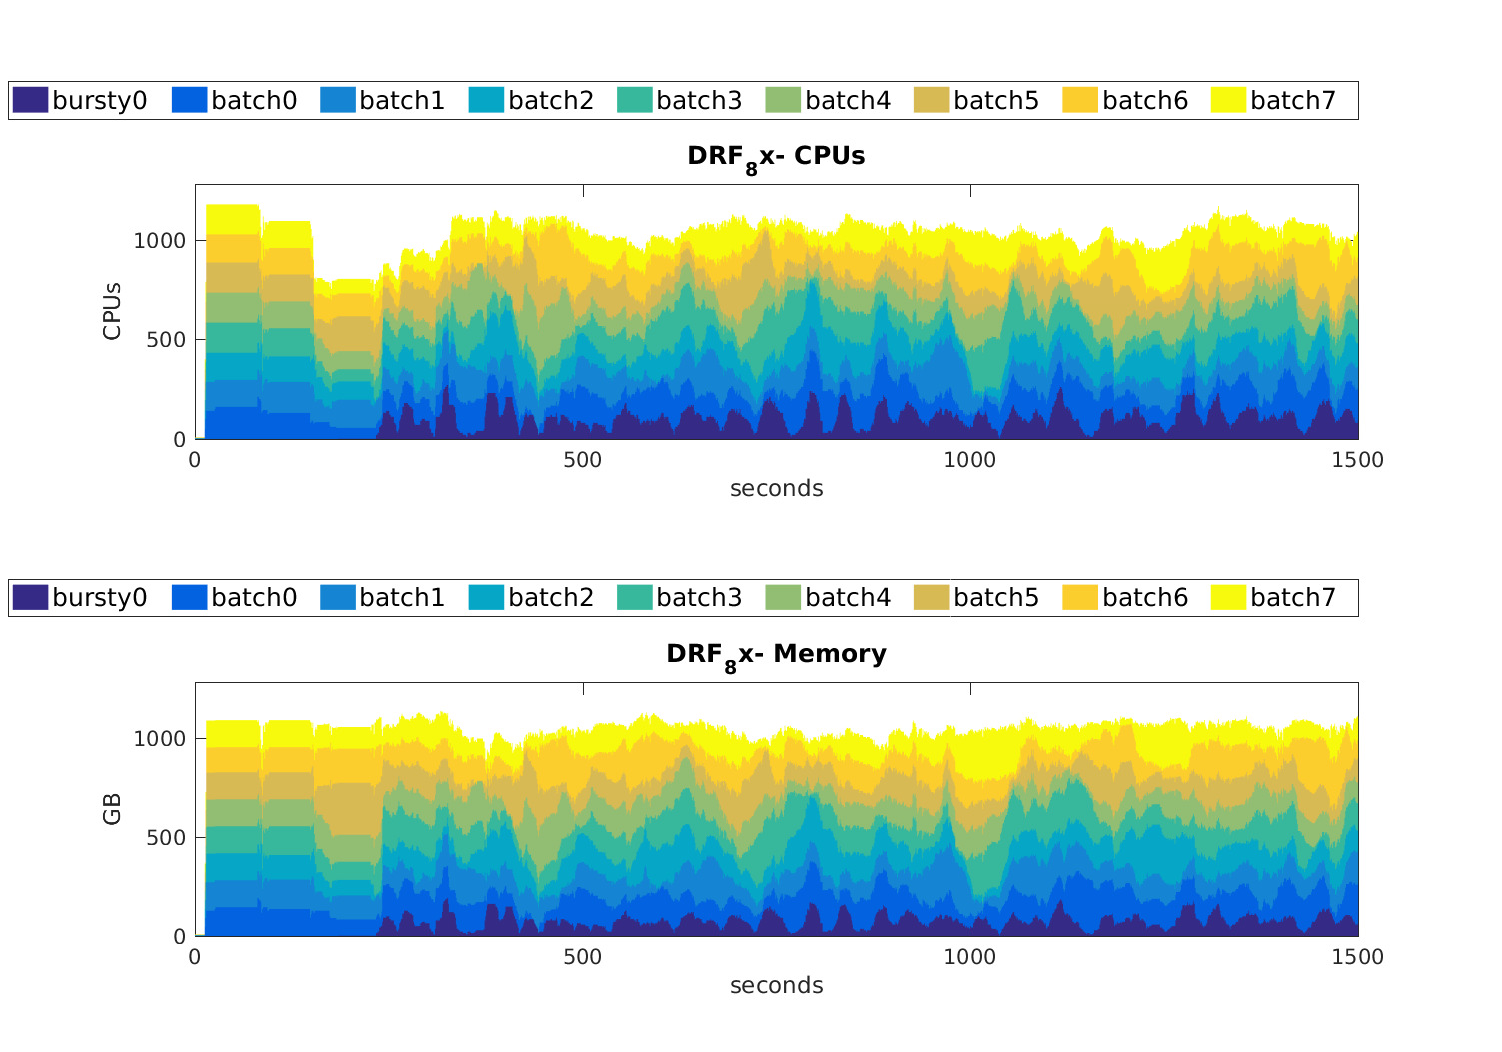
\includegraphics[width=1.0\linewidth]{fig/b8_res_usage_DRF_8x_BB}}
	\\
	\subfloat[Strict]{\includegraphics[width=1.0\linewidth]{fig/b8_res_usage_Strict_8x_BB}}
	\\	
	\subfloat[SpeedFair (\textbf{fixed})]{\includegraphics[width=1.0\linewidth]{fig/b8_res_usage_SpeedFair_8x_new_BB.pdf}}
	\caption{[Experiment] Details of the case of 8x on Figure \ref{fig:protecting_batch_jobs}. }
	\label{fig:protecting_batch_jobs_details}
\end{figure}


\begin{figure}[!t]
	\centering
	\subfloat[DRF]{\includegraphics[width=1.0\linewidth]{fig/b8_res_usage_DRF_BB}}
	\\
	\subfloat[Strict]{\includegraphics[width=1.0\linewidth]{fig/b8_res_usage_Strict_BB}}
	\\
	\subfloat[SpeedFair]{\includegraphics[width=1.0\linewidth]{fig/b8_res_usage_SpeedFair_BB}}
	\caption{[Experiment] Details of the case of 8 batch queues on Figure \ref{fig:busty_perf_grt}. }
	\label{fig:busty_perf_grt_details8}
\end{figure}


%\section{{(old)Results in 8-node cluster}}
\subsection{Setup}

We set up Yarn with \name on a cluster having 8 worker nodes on CloudLab. Totally, the cluster has 256 cpu cores, and 256 GB memory.

Yarn setting. 

We use the Facebook workload traces from SWIM \cite{SWIM} for batch jobs while interactive jobs are separately created. The SWIM workload include the MapReduce jobs to simulate the real workload in from a Facebook data center for 600 servers. However, SWIM workload does not have the information of demand on each resource dimension.  We generate the CPU and MEMORY demands as in Figure 1 of \cite{drf}. The batch jobs are CPU bound jobs. There CPU demand of a batch job is from 1 to 7 cpus while it mainly requires from 3GB to 4GB memory. 

%\todo{Need to choose the number of maps, and reduces as SWIM use the same number of maps and reduces for all jobs.}

\diff{We emulate the jobs using the BigBend workload traces. The details of resource usage are in Figure \ref{fig:b3_res_usage_SpeedFair_BB}. From the traces, we create the jobs that have the same structures, resource demand, and task durations. The jobs are encoded using TEZ and submitted to YARN for scheduling.}

\textbf{Bursty users' inputs}. To guarantee the bursty users' inputs, we first compute resource rate and duration that they require. We run only interactive jobs to estimate the completion time, and the average demand of them.
\begin{itemize}
	\item bursty jobs arrive in every 100 secs.
	\item On average, a bursty job having 2 phases (map and reduce) takes 30 secs to complete. As most of resources are used in the Map phase, we set the stage 1 duration at 20 secs as it requires a lot of resources for the first 20 secs for the map tasks. The resource rate for the stage 1 is 100\% of the cluster (256 GB, 256 vcores).
\end{itemize}

\textbf{Batch jobs queues.} All batch jobs are submitted at time $t=0$.

\subsection{resource usage in details}

\begin{figure}
\centering
\includegraphics[width=1.0\linewidth]{fig/swim_b3_res_usage_SpeedFair}
\caption{\textbf{Workload: SWIM (FB MapReduce)} \diff{Resource usage of using SpeedFair. There are 2 unexpected points in this figures: The overall resource utlization is a bit low and SpeedFair should have more resource. The resource utilization is a bit low because all batch jobs in a queue is scheduled in a FIFO manner so there are at most 4 jobs can run at the same time. Furthermore, every job requires a lot of resources in Map phase but very litte in Reduce phase. SpeedFair cannot be allocated more resources because of non-preemption. Please compare with the Strict method in Figure \ref{fig:swim_b3_res_usage_strict} for its correctness. } }
\label{fig:swim_b3_res_usage_SpeedFair}
\end{figure}

\begin{figure}
\centering
\includegraphics[width=1.0\linewidth]{fig/swim_b3_res_usage_Strict}
\caption{\textbf{Workload: SWIM (FB MapReduce)} \diff{Resource usage of using Strict. Strict actually uses DRF with a very high weight for the bursty queue. The weight of the root.bursty0 queue is set at 999999.}}
\label{fig:swim_b3_res_usage_Strict}
\end{figure}


\begin{figure}
\centering
\includegraphics[width=1.0\linewidth]{fig/b3_res_usage_SpeedFair_BB}
\caption{\diff{\textbf{Workload: BigBench (Tez). SpeedFair.} The resource usage of bursty jobs are not as high as in the simulation. What are the reasons behind this? Some reasons could be: non-preemption and slow start of tasks.}}
\label{fig:b3_res_usage_SpeedFair_BB}
\end{figure}

\begin{figure}
\centering
\includegraphics[width=1.0\linewidth]{fig/b3_res_usage_drf_BB}
\caption{\diff{\textbf{Workload: BigBench (Tez). DRF.} }}
\label{fig:b3_res_usage_drf_BB}
\end{figure}

\begin{figure}
\centering
\includegraphics[width=1.0\linewidth]{fig/b3_res_usage_Strict_BB}
\caption{\diff{\textbf{Workload: BigBench (Tez). Strict}}}
\label{fig:b3_res_usage_Strict_BB}
\end{figure}


\subsection{Bursty Regular jobs}

Figure \ref{fig:exp_interactive_compl_time} shows that \textbf{the completion time of jobs are not changed} when having more queues.

\begin{itemize}
	\item Graph type: bar chart.
	\item X-axis: Number of batch queues (1, 2, 4, 8).
	\item Y-axis: Completion time.
\end{itemize}

%\begin{figure}
%\centering
%\includegraphics[width=1.0\linewidth]{fig/exp_interactive_compl_time}
%\caption{(Old figure) Need to be updated}
%\label{fig:exp_interactive_compl_time}
%\end{figure}

\subsection{Bursty jobs with variant resource demand}

\textbf{Figure}: Interactive Job completion time for variant bursty jobs (optional)
\begin{itemize}
	\item Graph type: bar chart.
	\item X-axis: Number of batch queues (1, 3, 5, 8).
	\item Y-axis: Completion time.
\end{itemize}

\textbf{Figure}: Snapshot of Multiple Resource Allocation on Memory  Figure \ref{fig:res_usage_speedfair_exp}

%\begin{figure*}[!t]
%	\centering
%	\subfloat[DRF]{\includegraphics[width=1.0\linewidth]{fig/drf-vcore_usage}}
%	\\
%	\subfloat[SpeedFair]{\includegraphics[width=1.0\linewidth]{fig/SpeedFair-ram_usage}}
%	\caption{Resource Allocation in CPU (vcores)}
%	\label{fig:res_usage_speedfair_exp}2.5
%\end{figure*}

%\begin{figure*}[!t]
%	\centering
%	\subfloat[DRF]{\includegraphics[width=1.0\linewidth]{fig/drf-vcore_usage}}
%	\\
%	\subfloat[SpeedFair]{\includegraphics[width=1.0\linewidth]{fig/SpeedFair-ram_usage}}
%	\caption{Resource Allocation on Memory}
%	\label{fig:res_usage_speedfair_exp}
%\end{figure*}


\section{More Figures in details to debug}

What are the gaps between simulation and experiment.

\subsection{is slow-start the problem?}
\todo{Plot only bursty jobs to see what happens.}
\begin{figure}
\centering
\includegraphics[width=1.0\linewidth]{fig/b3_res_usage_SpeedFair_BB_bursty}
\caption{\diff{\textbf{Ony busry jobs. Workload : BigBench (TEZ).} } We can see the job is allocated resource slowly. We call this phenomenon ``slow start" }
\label{fig:b3_res_usage_SpeedFair_BB_only}
\end{figure}

\subsection{is non-preemption the problem?}
\todo{Use the short bursty jobs and batch jobs, to see what happen.}

\begin{figure}
\centering
\includegraphics[width=1.0\linewidth]{fig/b3_res_usage_SpeedFair_BB_1s}
\caption{\diff{\textbf{Uniform Workload (1 sec per task): BigBench (TEZ). SpeedFair}.} Since the task is too short and the tasks in the same stage do not start at the same time (\textbf{slow start}), the bursty jobs do not need the full capacity.}
\label{fig:b3_res_usage_SpeedFair_BB_1s}
\end{figure}

\begin{figure}
\centering
\includegraphics[width=1.0\linewidth]{fig/b3_res_usage_SpeedFair_BB_3s}
\caption{\diff{\textbf{Uniform Workload (3 sec per task): BigBench (TEZ). SpeedFair. This may have the same slow start prolem like 1sec uniform workload. However, we can see some impact from non-preemtion at 100, 600, ...} }}
\label{fig:b3_res_usage_SpeedFair_BB_3s}
\end{figure}

\begin{figure}
\centering
\includegraphics[width=1.0\linewidth]{fig/b3_res_usage_SpeedFair_BB_5s}
\caption{\diff{\textbf{Uniform Workload (5 sec per task): BigBench (TEZ).} }}
\label{fig:b3_res_usage_SpeedFair_BB_3s}
\end{figure}

\subsection{What else? May be Tez Scheduler?}



\newpage

\section{Work on the non-preemption and slow start issues}

\subsection{Enable preemption in Yarn}

We enable preemption in Yarn in Figure \ref{fig:b3_res_usage_SpeedFair_BB_preemption}. It has the same job profiles of Figure \ref{fig:b3_res_usage_SpeedFair_BB}. However, there is no significant improvement. The reasons may be: (1) \textbf{preempting a containter (for a task) is too slow}, (2) \textbf{allocating a containter (for a task) is too slow}. (1) is not the root cause as we already set preemption timeout at 100 ms, which kills a container to release the resource roughly in 100 ms. So, the speed of preemption is negligible. The slowly allocating a container for each task must be the problem here.


\begin{figure}
\centering
\includegraphics[width=1.0\linewidth]{fig/b3_res_usage_SpeedFair_BB_preemption}
\caption{\diff{\textbf{Preemption is ENABLED.} Workload: BigBench (TEZ).} Although the preemption is enabled, it is is not close to Figure \ref{fig:b3_res_usage_SpeedFair_BB_only}, it is NOT much better than Figure \ref{fig:b3_res_usage_SpeedFair_BB}.}
\label{fig:b3_res_usage_SpeedFair_BB_preemption}
\end{figure}

\textbf{Slowly allocating a container:} To confirm this, we run increase the duration of the every job of the bursty jobs 5x times. The results is detailed in Figure \ref{fig:b3_res_usage_SpeedFair_BB_5x}. Preemption helps the long-task duration bursty jobs here. In fact, the slowly allocating a container is  is related to the ``slow start'' issue.

\begin{figure}
\centering
\includegraphics[width=1.0\linewidth]{fig/b3_res_usage_SpeedFair_BB_5x}
\caption{\diff{\textbf{Preemption is ENABLED, task duration 5x.} Workload: BigBench (TEZ).} The preemption help bursty jobs when the task duration is much longer.}
\label{fig:b3_res_usage_SpeedFair_BB_5x}
\end{figure}


\subsection{Slow Start in Yarn}

The slow start issue is clearly shown in Figure \ref{fig:b3_res_usage_SpeedFair_BB_only}. When we run only a bursty job in the cluster, it takes 20 secs to reach the peak demand. In the first few seconds (7 secs in the figure), every job needs a single container (e.g., 1 cpu 1GB ram) for its application master (AM) (We can see when zoom the figure in.). This AM does the setup process in 7 secs but it is unavoidable. When the AM requests more resources, the demand is increasing reach to the peak demand next 13 secs (because the task duration of the first stage is 13 secs.). The similar slow start happens for the second bursty job in figure \ref{fig:b3_res_usage_SpeedFair_BB_5x}.

What is the root cause of slow start? The reason behind is that Yarn allocates the container (for a task) one by one to a single job. If the number of tasks is large, the slow start will have more negative impact on on our approach. Yarn has to allocate a container one by one to maintain the consistency of cluster distributed resources for multiple requests.

We implement the simulator for the larger clusters with larger workload.

\begin{itemize}
	\item DRF: 
	\item DRF-W: The weight of the interactive queue is set at 4.0 while others are 1.0.
	\item Strict Priority: Strict Priority is basically DRF-W in which the bursty queues have very high weights (e.g. positive infinity).
\end{itemize}


\noindent \textbf{Metrics:} Average completion time

\begin{itemize}
	\item How much does our proposed policy improve the performance?
\end{itemize}

\subsection{Job completion time improvement for short bursty jobs }


We run our algorithm and other baseline methods on 1 single bursty queue and a number of batch queues.

Figure \ref{fig:BB-compl_time} show the results of using Big bench workload. X-axis show the number of batch queues.
\begin{itemize}
\item The completion time of busty jobs are guaranteed as same as Strict's when the number of queues increases from 1 to 4. When the number of batch queues is 8, the bursty jobs cannot receive enough resources to complete in stage 1 because of non-preemption. In fact, there are many running jobs on the batch queues and we cannot just kill the running jobs to give more resources to the bursty jobs. When the number of (admitted) batch queues are more than 9, the algorithm does not admit the bursty queue.
\item The completion time of batch jobs are similar among 4 methods.
\item The completion time of batch jobs for all methods vary when we increase the number of batch queues as more batch jobs are in the cluster.
\end{itemize}

\begin{figure*}[!t]
	\centering
	\subfloat[bursty job's avg completion time]{\includegraphics[width=0.3\linewidth]{fig/BB-interactive_compl_time}}
	\subfloat[batch job's avg completion time]{\includegraphics[width=0.3\linewidth]{fig/BB-batch_compl_time}}
	\subfloat[Histogram of task durations]{\includegraphics[width=0.3\linewidth]{fig/BB-hist}}
	\\
	\subfloat[resources usage - Speedfair]{\includegraphics[width=1.0\linewidth]{fig/BB-b8_res_usage_speedfair}}
	\caption{[Simulation] Average completion time for Big Bench workload.}
	\label{fig:BB-compl_time}
\end{figure*}

Figure \ref{fig:TPC-H-compl_time} respectively show the simulation results of using TPC-H.
%\begin{itemize}
%\item Although the average bursty completion of DRF significantly increases, our method is not negatively impacted by the number of queues. The completion time is not as low as in the case of no batch queues because of non-preemption.
%\item The completion time of bursty jobs of SpeedFair are larger than Strict when the number of queues are greater than or equal to 8. The reasons behind this are non-preemption and the long task durations as in Figure \ref{fig:TPC-H-compl_time} (c). Some bursty jobs actually take longer than 50 secs to finish, which results in low resource allocation at stage 2. In the meantime, Strict asks for maximum resource any time.
%\item The completion time of batch jobs are not suffered as the batch jobs are very long.
%\end{itemize}

\begin{figure*}[!t]
	\centering
	\subfloat[bursty job's avg completion time]{\includegraphics[width=0.3\linewidth]{fig/updated.jpg}}
	\subfloat[batch job's avg completion time]{\includegraphics[width=0.3\linewidth]{fig/updated.jpg}}
	\subfloat[Histogram of task durations]{\includegraphics[width=0.3\linewidth]{fig/TPC-H-hist}}
	\caption{Average completion time for TPC-H workload.}
	\label{fig:TPC-H-compl_time}
\end{figure*}

Figure \ref{fig:TPC-DS-compl_time} show the output of running the algorithms on TPC-DS workload. The simulation results are expected for both bursty jobs and batch jobs.

\begin{figure*}[!t]
	\centering
	\subfloat[bursty job's avg completion time]{\includegraphics[width=0.3\linewidth]{fig/updated.jpg}}
	\subfloat[batch job's avg completion time]{\includegraphics[width=0.3\linewidth]{fig/updated.jpg}}
	\subfloat[Histogram of task durations]{\includegraphics[width=0.3\linewidth]{fig/TPC-DS-hist}}
	\caption{Average completion time for TPC-DS workload.}
	\label{fig:TPC-DS-compl_time}
\end{figure*}

\subsection{Batch jobs completion time when running long bursty jobs}

In Figure \ref{fig:BB-scaled_bursty}, we scaled the bursty jobs from 1 to 10 and observed how they affect the batch jobs.

\begin{itemize}
\item When the users submit very long bursty jobs, the batch jobs are starved and wait for all long bursty jobs to finish.
\item In the meantime, SpeedFair prevent the problem happen and allows batch jobs get resources.
\end{itemize}

\begin{figure}
\centering
\includegraphics[width=1.0\linewidth]{fig/BB-scaled_bursty}
\caption{[Simulation] SpeedFair can prevent the batch jobs from suffering the large bursty jobs. \todo{Reduce the duration of stage 1 or increase the number of batch jobs' tasks.}}
\label{fig:BB-scaled_bursty}
\end{figure}



{
\bibliographystyle{abbrv} 
\bibliography{bib/refs}
}

\end{document}
